\documentclass[10pt,a4paper]{article}

\usepackage[margin=1in]{geometry}
\usepackage[T1]{fontenc}
\usepackage{amsmath,amssymb,amsthm}
\usepackage{graphicx}
\usepackage{booktabs}
\usepackage{tabularx}
\usepackage{multirow}
\usepackage{array}
\usepackage{algorithm}
\usepackage{algpseudocode}
\usepackage{xcolor}
\usepackage{xurl}
\usepackage[numbers,sort&compress]{natbib}
\usepackage{hyperref}
\usepackage{enumitem}
\usepackage{caption}

\hypersetup{colorlinks=true, linkcolor=blue!50!black, citecolor=blue!50!black,
            urlcolor=blue!50!black}
\captionsetup{font=small, labelfont=bf}
\setlist{nosep, leftmargin=1.4em}
\sloppy
\emergencystretch=3em

\newtheorem{proposition}{Proposition}
\newtheorem{lemma}{Lemma}
\theoremstyle{remark}
\newtheorem{remark}{Remark}
\theoremstyle{definition}
\newtheorem{definition}{Definition}

\newcommand{\FF}{\mathbb{F}}
\newcommand{\ZZ}{\mathbb{Z}}
\newcommand{\Fb}{\mathcal{F}}
\newcommand{\Sem}[1]{S_{#1}}
\newcommand{\abs}[1]{\lvert #1 \rvert}
% A committed artefact in this repository; breakable anywhere.
\newcommand{\art}[1]{\path{#1}}
\newcommand{\cls}[1]{\textsc{#1}}

\title{Elliptic-Curve Index Calculus Against Pollard Rho:\\[4pt]
       {\large A Survey of Results, a Measured Frontier with Every Cost Priced,\\
       and Open Problems}}
\author{Anonymous}
\date{}

\begin{document}
\maketitle

\begin{abstract}
Index calculus is the method that, on paper, should exploit the most
structure in an elliptic-curve discrete-logarithm instance, and in practice
has never beaten Pollard rho on a prime-order curve of cryptographic shape.
Between July and mid-October 2026 we ran a sustained engineering and
measurement programme on this question in one open repository: about
6{,}900 commits and 450 dated study directories, the index-calculus part of
which began in the first week of September. This paper is the record of that
programme. We describe the routes we pursued---Frobenius-invariant factor
bases on Koblitz curves and their compact-orbit form; SAT and Gr\"obner-basis
decomposition oracles (matrix F4, F5, an inherited F4 and an F6-IC variant);
root-finding decomposition oracles; Kummer-tower and symmetry-reduced prime
and extension-field systems; isogeny and transfer routes; and a
twelve-workstream replication of the 2025--26 literature---the
infrastructure that made the results comparable (\emph{ecbench}, a native
harness that charges every ECDLP method in one counted unit, group-addition
equivalents per $\sqrt{r}$, with sealed records, exact replays, isolation
levels and paired cluster-bootstrap intervals), and what improved.

The largest single change came from a suggestion in a manuscript we
audited: the roots of Semaev's third summation polynomial in its free
variable are $x(R+F)$ and $x(R-F)$, so a two-summand decomposition needs no
polynomial system at all. We proved this (also in Lean), generalised it to
meet-in-the-middle pair-sum tables for three and four summands, to a CUDA
kernel, to Kummer-tower bases and to dense root indices, and built it into
the harness. Per decomposition it is $383$--$1{,}535\times$ faster than our
matrix F4 on Koblitz curves and $3{,}021$--$5{,}802\times$ faster than
Buchberger on the five NIST prime curves; end to end it is
$50$--$105\times$ faster than msolve on small prime curves. Inside ecbench
it moved the best complete-count Koblitz index-calculus arm at $n=13$ from
$S=38.8$ to $S=23.0$, below an XOR-priced F4 at $S=421$ but still
$1.55\times$ the strong signed-Frobenius rho. FGHR's $D_4$ symmetry cut the
$k=4$ Gaudry solve over $\FF_{p^4}$ by $47.5$--$48.4\times$, moving a
modelled crossover with rho from $2^{150}$ to $2^{135}$; our $\FF_p$ F4
reached parity with msolve on square systems; and a compact-orbit Koblitz
index calculus with retained precomputation solves one unseen public target
at $n=61$ $13.9\times$ faster online than rho (95\% interval $9.8$--$19.1$,
64 targets, pinned host) while costing $83\times$ rho when its set-up is
charged. We report the negative results with the same weight: no measured
index-calculus arm beats matched rho on the cold, one-target,
set-up-inclusive boundary; a group-homomorphic transfer cannot change
decomposition counts (we state the conservation lemma); and several
literature claims did not survive implementation. Every number cites a
committed artefact; nothing here concerns a deployed curve or key recovery.

\end{abstract}

\tableofcontents
\bigskip

\section{Introduction}\label{sec:intro}

For a prime-order subgroup $\langle G\rangle$ of size $r$ on an elliptic
curve $E/\FF_q$, the best generic algorithm for the discrete-logarithm
problem is Pollard rho~\cite{pollard1978,vanoorschot1999}, with expected
cost $\sqrt{\pi r/(2A)}$ group operations when $A$ automorphisms (negation,
and on a Koblitz curve the Frobenius) can be folded into the
walk~\cite{wiener1998,gallant2000}. Index calculus, the method that breaks
finite-field discrete logarithms in subexponential time, was brought to
elliptic curves by Semaev's summation polynomials~\cite{semaev2004} and by
Gaudry's and Diem's analyses over extension
fields~\cite{gaudry2009,diem2011}. Its open question has always been
\emph{where the crossover is}: on which curves, at which sizes and under
which accounting does it cost less than rho?

This paper documents fourteen weeks (1 July--14 October 2026) of work on
that question in one repository. The index-calculus programme proper ran
from 6 September to 14 October; July and August hold the preceding
prime-field structure work that motivated it
(\S\ref{sec:chronology}). The output is large: about 6{,}900 commits,
about 450 dated study directories under \art{research/}, 27 rows of the
performance index \art{benchmarks/README.md}, a boundary ledger
(\art{docs/ic/boundary_targets.json}), a native measurement harness
(\art{src/cryptanalysis/ecbench/}), and a companion manuscript on
root-finding decomposition (\art{papers/rootfinding-decomposition/}). It
is easy, in a body of work this size, to improve a headline number by two
orders of magnitude and establish nothing; this paper is organised to
prevent that. Every improvement is stated with the boundary on which it
was measured (oracle stage, complete solve, cold one-target cost, online
cost after retained set-up), the unit, the sample, the interval, and the
committed artefact that holds the records.

\paragraph{The routes.} We pursued six lines, each a section below:
\begin{enumerate}
\item \emph{Root-finding decomposition} (\S\ref{sec:rootfinding}):
  replacing the Gr\"obner solve of the decomposition step by closed-form
  roots of $\Sem3$, then by meet-in-the-middle tables for more summands,
  then by GPU, tower and dense-index variants.
\item \emph{Gr\"obner-basis engines} (\S\ref{sec:groebner}): matrix F4,
  F5, an inherited F4 that re-uses its root echelon form, an
  index-calculus-specific F6-IC, an $\FF_p$ F4 brought to msolve parity,
  and an audit that found and fixed one soundness bug.
\item \emph{Koblitz and binary curves} (\S\ref{sec:koblitz}):
  Frobenius-invariant factor bases~\cite{ggmp2020}, their compact
  signed-orbit form, SAT oracles~\cite{trimoska2020}, and a ladder of
  one-target online comparisons with rho from $n=53$ to $n=83$.
\item \emph{Prime and extension fields} (\S\ref{sec:prime}): $j=0$ and
  $a=-3$ known-answer ladders, the Kummer-tower factor base of
  Petit--Kosters--Messeng~\cite{pkm2016}, and Gaudry's $k=4$ index
  calculus over $\FF_{p^4}$ with the $D_4$ symmetry of
  Faug\`ere--Gaudry--Huot--Renault~\cite{fghr2014}.
\item \emph{Isogeny, transfer and structure routes}
  (\S\ref{sec:transfer}): conductor gaps in the ECC2K-130 isogeny class,
  isogeny fibres, transfer-aware index calculus, GHS and Weil descent;
  mostly negative, with one lemma that explains why.
\item \emph{Literature replication} (\S\ref{sec:prime},
  \S\ref{sec:transfer}): the \emph{lit2026} programme, which turned each
  finding of a 2025--26 literature search into a measured change, a
  diagnostic, or a recorded negative.
\end{enumerate}
Underneath all six sits the measurement work of \S\ref{sec:method}: a
single harness (\emph{ecbench}) that charges rho, BSGS, the kangaroo and
index calculus in one unit on one-target workloads, and the accounting
corrections that the harness forced on earlier claims.

\paragraph{Contributions.}
\begin{itemize}
\item A unit and a boundary: $S=\text{group-addition
  equivalents}/\sqrt{r}$, cold one-target with every phase charged, beside
  a separately reported online window; sealed, replayable records; and a
  frontier definition under which two numbers are comparable only when
  every component of the measurement domain matches
  (\S\ref{sec:method}).
\item Root-finding decomposition taken from an observation to an
  engineered, verified, harness-integrated oracle family, with a
  machine-checked proof of the identity it rests on
  (\S\ref{sec:rootfinding}).
\item A documented map of which levers move a constant, which move nothing,
  and which make things worse, across about 40 measured variants of the
  decomposition, factor-base and linear-algebra stages
  (Table~\ref{tab:improvements}).
\item An honest frontier (\S\ref{sec:frontier}): the cold one-target
  frontier is still rho; the retained-set-up online frontier has an
  admitted index-calculus point; the stage frontier moved substantially.
\end{itemize}

\paragraph{What this paper does not claim.} No asymptotic sub-rho
algorithm, no change to the Gaudry--Diem picture for prime fields, no
statement about ECC2K-130, P-256 or any deployed curve beyond labelled
arithmetic on public parameters, no key recovery. Every instance is a
public synthetic or standard-parameter known-answer instance. Every change
is classed, in the repository's vocabulary, as an \cls{advance} (an
exponent or a crossover moves under complete accounting),
\cls{engineering} (a constant moves), \cls{relabelling}, or
\cls{accounting}; with one modelled exception (\S\ref{sec:gaudry}) every
improvement in this paper is \cls{engineering} or \cls{accounting}.

\paragraph{How to read the numbers.} ``$X\times$'' always means
baseline cost divided by candidate cost on the stated boundary. Stage
ratios (one decomposition, one Gr\"obner call) are never presented as
end-to-end speed-ups; wall-time ratios from hosts that did not earn an
isolation level are labelled \emph{descriptive}; a cost with unpriced work
is labelled a \emph{lower bound}. Appendix~\ref{app:artefacts} lists the
artefact behind each table.

\section{Background}\label{sec:background}

\paragraph{Rho and its floor.} With $A$ efficiently computable
automorphisms acting on $\langle G\rangle$, a rho walk on orbit
representatives has expected cost $\sqrt{\pi r/(2A)}$ group additions.
$A=2$ (negation) on every curve; $A=2n$ on a Koblitz curve
$y^2+xy=x^3+ax^2+1$ over $\FF_{2^n}$, where the Frobenius
$\pi(x,y)=(x^2,y^2)$ acts on $\langle G\rangle$ as a scalar
$\lambda$~\cite{wiener1998,gallant2000}. ECC2K-130 is the case $a=0$,
$n=131$ of this family; its record GPU rho attempt is a separate paper in
this repository (\art{paper/ecc2k130/}).

\paragraph{Index calculus on elliptic curves.} Fix a factor base
$\Fb\subset E(\FF_q)$. A \emph{relation} is a decomposition
$aG+bQ=R=P_1+\cdots+P_m$ with $P_i\in\Fb$; once about $\abs{\Fb}$ relations
are found, linear algebra over $\ZZ/r$ yields $\log_G Q$. The pipeline has
five stages (factor base, decomposition oracle, relation yield, rank/linear
algebra, verification) and a sixth, the comparison with rho on the same
target. The \emph{decomposition oracle} decides whether $R$ splits over
$\Fb$. Semaev~\cite{semaev2004} reduced it to the roots of the summation
polynomial $\Sem{m+1}(x_1,\ldots,x_m,x_R)$, which vanishes exactly when
$\pm P_1\pm\cdots\pm P_m=R$ for points with those abscissae. Over
$\FF_{2^n}$ or $\FF_{p^k}$ the factor base is chosen as the points whose
abscissa lies in a subspace or subfield, and Weil restriction turns
$\Sem{m+1}=0$ into a polynomial system over the base field; the textbook
oracle solves that system with a Gr\"obner-basis engine (F4/F5,
\cite{faugere1999,faugere2002}) or a SAT solver~\cite{trimoska2020}.
Gaudry~\cite{gaudry2009} and Diem~\cite{diem2011} give the asymptotics
over extension fields; for prime fields no factor base is known that makes
the method competitive, and summation-polynomial systems over $\FF_p$ are
the subject of the Kummer-tower and rational-map bases of
Petit--Kosters--Messeng~\cite{pkm2016}.

\paragraph{Frobenius-invariant bases.} Galbraith, Granger, Merz and
Petit~\cite{ggmp2020} observe that a factor base with $\pi(\Fb)=\Fb$ splits
into Frobenius orbits of size dividing $n$, with
$\log\pi^k(P)=\lambda^k\log P$. The unknowns collapse by $\approx n$, the
matrix by $\approx n^2$, and ordered decompositions save $m!$---more than
rho's $\sqrt{2n}$, but from a base too far behind to overtake it at
deployed sizes. Invariant bases come from linearised polynomials attached
to the factors of $x^n-1$ over $\FF_2$; the subspace dimension is
$\ell=\operatorname{ord}_n(2)$, so the base size is fixed by $n$
(Table~1 of \art{RESEARCH_KOBLITZ_INDEX_CALCULUS.md}).

\paragraph{Symmetries of the system.} The decomposition system is
invariant under the symmetric group $S_m$; rational 2-torsion adds sign
changes, and Faug\`ere, Gaudry, Huot and Renault~\cite{fghr2014} show that
in the coordinate $Y$ with $Y(P+T)=-Y(P)$ the invariance group becomes the
Weyl group $D_m$, with a much smaller quotient. We measure this at $m=4$
in \S\ref{sec:gaudry}.

\section{The theory, by field type}\label{sec:theory}

% Survey section (draft 2026-10-15). Sources: LITERATURE.md; every
% statement below is at abstract level until the full papers are read.

\subsection{What a decomposition costs}

Every index-calculus algorithm for elliptic curves in the literature
spends its time in three places: finding about $\abs\Fb$ relations (each
a decomposition of a random combination $aG+bQ$ over $\Fb$), solving the
sparse linear system over $\ZZ/r$, and, in some variants, a descent of
the target. The second and third are well understood. The first is the
crux: a uniformly random point decomposes over a base of size $N$ into $m$
summands with probability about $N^m/(m!\,r)$, so relations need about
$m!\,r/N^{m-1}$ trials, and each trial costs whatever the decomposition
oracle costs. Every result below is a statement about one of three things:
how large $N$ can be while membership stays algebraically testable, how
cheap the oracle is, and how the two trade against the linear algebra.

\subsection{Extension fields $\FF_{q^k}$ with $k>1$ fixed or small}

Gaudry~\cite{gaudry2009} takes $\Fb$ to be the points with abscissa in the
base field $\FF_q$ and decomposes into $m=k$ summands by Weil restriction of
$\Sem{k+1}$, a system of $k$ equations in $k$ unknowns over $\FF_q$. For
fixed $k$ this gives $\tilde O(q^{2-2/k})$, asymptotically below rho's
$q^{k/2}$ for $k\ge3$; the constant hidden in the Gr\"obner solve grows
very quickly with $k$, which is what makes the crossover large in
practice (to be quantified from the paper).
Diem~\cite{diem2011} extends the analysis to families where $k$ grows,
proving subexponential complexity over sequences of fields with suitably
balanced $q$ and $k$. Joux and Vitse's work on decomposition and cover
attacks over small extension fields is to be added here once read. FGHR~\cite{fghr2014} exploit the action of $S_m$ and of
the 2-torsion to replace $\Sem{m+1}$ by its invariant form, cutting the
Gr\"obner work by large factors; our measurement at $k=4$
(\S\ref{sec:gaudry}) is a direct instance.

\subsection{Binary fields $\FF_{2^n}$ with $n$ prime}

Prime $n$ leaves no subfield, so the factor base is taken to be the points
whose abscissa lies in an $\FF_2$-vector subspace $V$ of dimension $\ell$.
Weil restriction then gives a quadratic-to-low-degree Boolean system whose
difficulty is governed by its degree of regularity. The whole debate about
binary curves is a debate about that degree.

\paragraph{The subexponential claims.} Petit and
Quisquater~\cite{petit2012} conjectured, from experiments and heuristic
evidence, that these systems have degrees of regularity only slightly above
the degrees of their equations (the \emph{first fall degree assumption}),
and deduced a heuristic $2^{c\,n^{2/3}\log n}$, $c<2$, for a variant of
Diem's algorithm, beating generic methods only for $n\gtrsim2000$.
Semaev~\cite{semaev2015} split summation polynomials into cubic Boolean
systems, argued for regularity degree at most 4 under the same kind of
assumption, and obtained a heuristic $2^{c\sqrt{n\ln n}}$ with
$c\approx1.69$; its first version concluded that several FIPS binary curves
fall faster than Pollard rho, a conclusion its revision says does not hold
under the weaker assumption that the regularity degree is
$o(\sqrt{n/\ln n})$.

\paragraph{The evidence against.} Shantz and Teske~\cite{shantz2013}
tested the Petit--Quisquater heuristics experimentally. Huang, Kosters and
Yeo~\cite{hky2015} introduced the \emph{last fall degree}, independent of
the monomial order, gave computational evidence against the first fall
degree assumption in characteristic~2, and constructed summation-polynomial
Weil descent systems where it is unlikely to hold. Galbraith and
Gebregiyorgis~\cite{galbraith2014} improved the variable choice (binary
Edwards curves), found symmetry-breaking factor bases and SAT solvers
inconclusive, and concluded that rho remains much faster for prime-degree
binary fields of reasonable size. The Galbraith--Gaudry
survey~\cite{galbraith2016} reaches the same verdict for characteristic-two
curves over prime-degree fields.

\paragraph{Where it stands.} No proof or refutation of a subexponential
algorithm for prime-degree binary curves exists. The open quantity is the
solving degree of Weil-descended $\Sem{m+1}$ as $n$ and $m$ grow; recent
work supplies diagnostics (saturation-exponent bounds, multi-graded
regularity, tests for where systems stop looking generic) but no bound for
these systems. Our own registered refutation-degree law at $m=3$
(\S\ref{sec:groebner}) is one data point and ended inconclusive.

\subsection{Subfield (Koblitz) curves}

When the curve is defined over $\FF_2$ the Frobenius acts on the group,
and Galbraith, Granger, Merz and Petit~\cite{ggmp2020} show that a
Frobenius-invariant factor base saves a factor $\approx n$ in relations and
$\approx n^2$ in linear algebra---more than rho's $\sqrt{2n}$---while
concluding that Koblitz-curve security is not threatened at deployed sizes.
Our Koblitz work (\S\ref{sec:koblitz}) builds on this.

\subsection{Prime fields}

Over $\FF_p$ there is no subfield and no subspace, and no factor base is
known for which membership is both dense enough and algebraically testable.
Semaev's original small-abscissa base leads to systems of very high degree.
Petit, Kosters and Messeng~\cite{pkm2016} construct bases from rational maps
(including the Kummer tower $\mu_{2^t}$) that give the summation system
extra structure; Amadori, Pintore and Sala~\cite{aps2018} build the base
from the instance and need only one relation search, improving on both;
McGuire and Mueller~\cite{mcguire2017} avoid Gr\"obner bases altogether by
fast evaluation of $\Sem m$ through iterated resultants, and in a second
variant by summing $m-1$ factor-base points and testing membership of the
result---the same mechanism as the two-summand root-finding oracle of
\S\ref{sec:rootfinding}. All of these remain exponential and slower than
rho; a 2024 analysis again concludes that no subexponential prime-field
method is known.

\subsection{Lower bounds}

Generic-group lower bounds bound everything that does not use curve
structure. With preprocessing, Corrigan-Gibbs and
Kogan~\cite{cgk2018} show $S\,T^2=\tilde\Omega(\varepsilon N)$ for $S$ bits
of advice and online time $T$; this is the bound against which the
retained-set-up (online) results of \S\ref{sec:koblitz} must be read. A
2026 structured-generic-group bound shows that an algorithm exploiting
structure on only a $\delta$ fraction of elements needs
$\Omega(\min(\sqrt q,1/\delta))$ time---for index calculus, the
decomposable set must be dense \emph{and} cheaply testable.

\section{Measuring index calculus against rho}\label{sec:method}

The programme's first lesson was that index-calculus numbers from
different studies did not compose: one study timed a decomposition, another
a relation, a third a whole multi-target batch with shared tables, each on
a different host and in a different unit. Four mechanisms, built in this
order, fixed that.

\subsection{The boundary ledger (10 September)}

\art{docs/ic/BOUNDARY_TARGETS.md} and its machine twin
\art{docs/ic/boundary_targets.json} give each regime (Koblitz, binary,
prime) and each pipeline stage (\texttt{factor\_base},
\texttt{decomposition}, \texttt{relation\_yield}, \texttt{rank},
\texttt{end\_to\_end\_dlp}, \texttt{vs\_rho}) a current record, a next
target and acceptance gates. A row promotes only when its evidence JSON
carries every field the measurement schema requires for that stage---for
example, a \texttt{decomposition} claim that beats an algebraic frontier
must report the first-fall degree, and a \texttt{vs\_rho} claim needs one
target, the identical public point for both methods, verified scalars,
five exclusive IC online phases, the automorphism discount, matched
resources and a host-isolation receipt. Missing fields fail closed. The
primary \texttt{vs\_rho} question is the online cost of \emph{one}
previously unseen target after reusable IC preparation; multi-target and
amortised results are secondary and must be declared as such.

\subsection{ecbench (from 2 October)}\label{sec:ecbench}

\emph{ecbench} (\art{src/cryptanalysis/ecbench/}, \art{src/bin/ecbench.rs},
documented in \art{docs/ecbench/README.md}) runs every ECDLP method behind
one interface, on the same single-target workloads, in one unit, into
sealed records.

\paragraph{Unit.}
\[
  S \;=\; \frac{\text{total group-addition equivalents (GAE)}}{\sqrt r},
  \qquad
  S_{\text{floor}}=\sqrt{\pi/(2A)}.
\]
An addition or doubling is one GAE; a scalar multiplication is charged as
the additions it performs; native work (lookups, row operations, square
roots, Artin--Schreier solves, word XORs) is priced at a pinned conversion
where the repository has one and is otherwise recorded as
\emph{uncharged}, which marks the record's $S$ as a \emph{lower bound}.
Plain rho has $S\approx1.25$.

\paragraph{What a measurement is.} One workload is one curve, subgroup,
generator and target; nothing survives between executions, so every table
a method builds is inside its cost (\emph{cold}). Beside the cold $S$
every record carries the one-target \emph{online window}, split for index
calculus into the five exclusive phases \texttt{target\_query},
\texttt{target\_PDP}, \texttt{target\_relation\_check},
\texttt{target\_descent}, \texttt{target\_recovery\_check}. Targets are
either planted or \emph{public}---hashed to the subgroup so that nobody
knows the logarithm---and the runner verifies $[k]G=Q$ in its own process;
\texttt{ecbench verify} checks it again from the files. Failed, exhausted
and timed-out runs are rows, never dropped.

\paragraph{Identity, sealing and replay.} Every object (curve, factor
base, method parameters, spec, session, host environment class) is named by
a hash of what it is (\texttt{ECBS1h\ldots} for sessions,
\texttt{ECBND1h\ldots} for bounds). Each execution appends one sealed
record; \texttt{ecbench verify} replays measured records and emits an audit
receipt whose SHA-256 is the replay certificate. Operation counts are
deterministic, so a replay must match to the last digit; a mismatch is
preserved as a failed audit (\S\ref{sec:corrections}).

\paragraph{Isolation.} A run earns L0 (recorded under a host capsule), L1
(pinned, affinity read back, no foreign SMT sibling, CPU/wall $\le1.05$),
L2 (quiet: zero steal, foreign busy time $\le1\%$, run-queue delay
$\le0.5\%$, $\le50$ preemptions/s) or L3 (isolated cores, fixed governor,
bare metal). Wall time is admitted only at the spec's required level
(default L2) with at least five admitted pairs and an A/A interval;
otherwise it is printed as \emph{descriptive}. Operation counts need no
isolation. macOS hosts earn L0; a GitHub-hosted runner earned L1 on 72/72
runs and matched a macOS session's operation counts to the last digit.
\emph{isolab} prepares lab hosts for L3 and cross-host replay.

\paragraph{Statistics.} The comparable statistic is the mean $S$ (the
floor is an expectation). Comparisons are paired by (workload, round) with
shared seeds, reported as a ratio of totals $\sum S_B/\sum S_A$, never a
mean of ratios, with a two-stage cluster bootstrap that resamples
workloads, then pairs. An operations A/A is exactly 1 by construction and
checks determinism. A claim about scaling fits exponents over at least
four sizes.

\paragraph{Bounds and the frontier.} \texttt{ecbench} also records sealed
\emph{bounds}---constant and exponent with intervals, per phase---and a
challenge protocol whose verdict says whether a candidate advances,
trades, matches or regresses an incumbent and at which level (exponent,
constant, primitive). The incumbent for cold one-target Koblitz operations
is \texttt{rho.signed\_frobenius\_strong} (bound
\texttt{ECBND1h05a2ea918f3c}): $1.089\times$ the floor $[0.927,1.261]$,
fitted exponent $\alpha=0.451$ $[0.399,0.512]$, 144 runs at six sizes
(\art{research/ecbench_frontier_20261013/}).

\begin{definition}[comparability]\label{def:domain}
A performance point is keyed by the tuple
\begin{align*}
D=\bigl(&\text{curve and subgroup},\ \text{target law},\
  \text{cold}\mid\text{online}\mid\text{stage},\ \text{unit and unpriced work},\\
  &\text{set-up amortisation }q,\ \text{memory envelope},\
  \text{correctness/replay/isolation class}\bigr).
\end{align*}
Two points are ratio-comparable only when every component of $D$ except
the method matches; a method is on the frontier of a domain when no admitted point is
no worse on every axis and strictly better on one.
\end{definition}
\noindent This rules out the four collapses we saw most often: online wall
as cold cost; word XORs, probes, field operations and GAE as
interchangeable; a lower bound as a complete cost; an L0 wall ratio as an
admitted speed-up.

\subsection{The pricing band}\label{sec:band}

Almost no cost in a record is complete, and the rho baselines are no
exception. Rho, BSGS and the kangaroo leave canonicalisations, partition
hashes and table inserts and lookups unpriced. An index-calculus arm is
complete only on curves that have a pinned timing calibration
(\art{docs/ic/calibration.json}), which converts lookups, row operations,
Artin--Schreier solves, Frobenius maps and solver word XORs to GAE at
measured ratios of roughly $10^{-3}$ to $10^{-1}$. A ``complete'' index
calculus set against a lower-bound rho is therefore lopsided, and several
earlier comparisons in this repository were of that kind.

Since 15 October every cross-method comparison uses a \emph{pricing band}
(repository rule, \texttt{AGENTS.md} \S5a; native implementation
\texttt{ecbench band}). For a record with charged cost $G$, calibration-priced
native cost $C$ over $n_C$ operations, and $U$ operations behind its
unpriced counters,
\[
  S(w)=\frac{G-C+w\,(U+n_C)}{\sqrt r},\qquad w\in\{0,\ 0.1,\ 1\}
  \text{ GAE per native operation},
\]
applied alike to every arm, references included. Two arms are ranked only
if their order is the same at every weight; otherwise the pair is reported
as unresolved. An arm that names an unpriced counter without counting it is
a lower bound and cannot be ranked. The band brackets the pinned
calibrations from below and above, so a ranking that survives it does not
depend on the host the calibration came from.

\subsection{Claim hygiene and change classes}

Every study directory states a protocol before it runs (frozen inputs are
committed first), keeps failures, and closes with a decision in one of the
four classes of \S\ref{sec:intro}. A controlled-experiment rule requires a
negative control from the right null population, a positive control that
proves the detector can see the effect, and the same instrument on every
arm before any comparative statement. Blockers are recorded as named
problems (\art{problems/}) with exit criteria rather than silently dropped.
Measurement code is native (Rust); Python only lays out recorded values.

\subsection{Corrections the accounting forced}\label{sec:corrections}

Building the harness and the ledger exposed errors in earlier claims,
including our own. We list them because they change how earlier numbers
must be read.
\begin{enumerate}
\item \emph{Online Koblitz ratios relabelled} (7--8 October,
  \art{docs/ic/PLAN_IC_ACCOUNTING_FIXES_20261007.md}). Same-point online
  ratios of $124.85\times$ ($n=61$), $2{,}864.1\times$ ($n=71$),
  $1{,}189.7\times$ ($n=73$) and $8.2\times$ ($n=83$) had verified answers
  but no host-isolation receipt; they are \emph{exploratory}. Only the
  later 64-target pinned panel at $n=61$ is admitted (\S\ref{sec:koblitz}).
\item \emph{ECC2K-130 extrapolation constants corrected}
  (\art{RESEARCH_ECC2K130_IC_FEASIBILITY.md}): the structural model
  predicts $C=0.25$ in $\text{probes/relation}\approx C\,r/(n^2K^2)$; the
  fitted $C$ is $0.27$ at $n=61$ but $1.2$--$1.5$ at $n=71,73$, an
  unexplained gap now stated rather than absorbed.
\item \emph{``F4'' that was Buchberger}
  (\art{research/ecbench_rootfinding_assessment_20261012/REPORT.md}): the
  NIST benchmark of the root-finding manuscript printed its baseline as F4
  but called \texttt{groebner\_f4::buchberger}; its $3{,}021$--$5{,}802\times$
  are ratios to Buchberger. The manuscript's claim that no implementation
  can use fewer than linear field operations per ideal is too broad once a
  reusable pair table is allowed.
\item \emph{Unpriced word XORs} (\art{research/ecbench_rootfind_faster_20261014/}).
  Inherited F4's Boolean word XORs were counted but not charged, so its
  $S=16.7$ at Koblitz $n=13$ was a lower bound that looked competitive
  with rho ($14.4$). Pricing them gives $S=421.4$.
\item \emph{Cross-host counter drift}
  (\art{research/ecbench_frontier_20261013/audits/}): a replay-all audit
  of the root-finder session on x86\_64 matched 120/168 records; all 48
  inherited-F4 rows differed in solver word-XOR counts (e.g.\ 301{,}961
  versus 300{,}531), with every scalar, trial count and charged GAE
  unchanged. The failed receipt is kept; the F4 stage comparison is
  historical until the drift is explained.
\item \emph{A soundness bug} (\art{docs/ic/GROEBNER_F4F5F6_AUDIT_20261010.md}
  \S2.1): a degree-bounded \texttt{f4\_fp::solve} could certify solutions
  of an inconsistent system (over $\FF_5$, $\{x^3+1,xy-1,x+y\}$ returned
  two ``solutions''). Fixed by evaluating every candidate on the input.
\item \emph{F6-IC charged cost} (\S\ref{sec:groebner}): a stage win in
  word XORs became a $64.6$--$1{,}353\times$ loss in charged $S$ once its
  batched geometry was counted---recorded as an accounting result, not an
  advance.
\item \emph{Lopsided pricing} (\S\ref{sec:band}): comparisons of a
  calibration-priced index calculus with a lower-bound rho. On the
  frontier campaign's train panel at Koblitz $n=13$ the compact-orbit arm,
  earlier quoted at $1.08\times$ rho as a lower bound, is $0.93\times$,
  $1.53\times$ and $5.7\times$ the strong rho at $w=0$, $0.1$ and $1$
  (columns 2, four train targets,
  \art{research/ic_frontier_campaign_20261015/select/SELECTION.md}): below
  rho with native work free, above it otherwise, so the pair is unresolved
  inside the band rather than a win for either side.
\end{enumerate}

\section{Chronology}\label{sec:chronology}

Figure~\ref{fig:timeline} shows commit activity on \texttt{main} by ISO
week. Theme lines are case-insensitive keyword matches on commit subjects
(a commit may match several themes or none; the regular expressions are in
the paper's \texttt{README.md}), so they indicate where effort went, not
how much of it was index calculus. The grey bars include unrelated work in
the same repository (the ECC2K-130 GPU rho campaign, an isogeny KEM,
post-quantum benchmarks), which dominates week 37.

\begin{figure}[t]
\centering
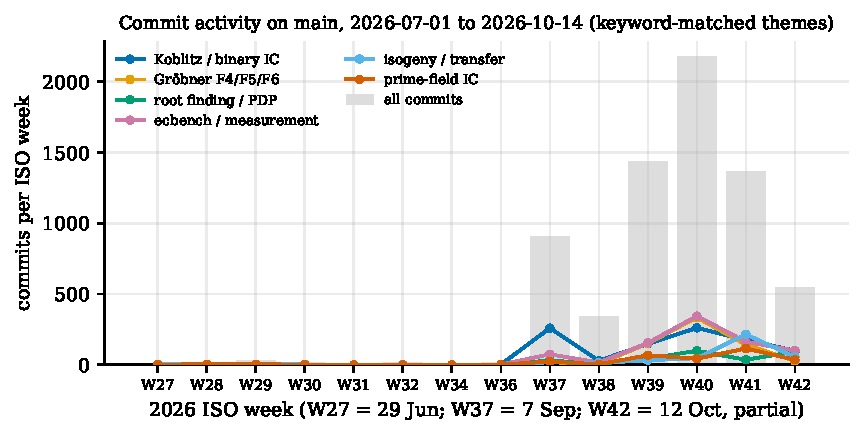
\includegraphics[width=\linewidth]{figures/fig-timeline.pdf}
\caption[]{Commits per ISO week on \texttt{main}, 1 July--14 October 2026
(6{,}882 commits; week 42 partial). Lines: commits whose subject matches
each theme's keywords. Source: \texttt{git log} at the paper's base commit;
values in \art{figures/data.json}.}
\label{fig:timeline}
\end{figure}

\paragraph{Prelude: July and August.} The prime-field \emph{ecdlp
autolab} ran numbered threads on curve structure---universal order-2
Frobenius forms, the CM-73 family $\{19,37,79,109\}$, sextic-twist pairs
that are Howe-glueable (5 of 15)---and its draft ``An Empirical
Resistance Map for Prime-Field ECDLP''
(\art{research/ecdlp_autolab/PAPER_DRAFT.md}). Those threads found
structure but no solver advantage, which is what turned the programme
towards index calculus, where structure is supposed to pay.

\paragraph{Phase 1, 6--14 September: Koblitz index calculus from
scratch.} The ECC2K-130 rho client and an audit of a public
index-calculus benchmark's SAT/UNSAT labels (6 Sept) were followed by
Frobenius-invariant factor bases with a matrix-F4 Semaev oracle, an
XOR-native SAT oracle after Trimoska et al.\ (7 Sept), and a $\sim50\times$
faster Semaev solve the same day. On 8 September a scaling experiment
showed the SAT route does not scale and that the refutation frontier
belongs to F4; pairs-and-solve replaced triple enumeration for
$\Sem4$. The boundary ledger was codified on 10 September, together with
a meet-in-the-middle oracle, incremental modular linear algebra and a
CADO-style split into factor-base logs then descent. A burst of more than
100 numbered pipeline stages (12--13 Sept: PCLMUL field products, fused
pair collection, scalar-blind targets, rank-aware scans) took the
multi-target $n=53$ pipeline to a 1{,}024-target process-wall crossover
against batched rho. On 13--14 September six pre-registered ECC2K-130
decomposition experiments ran (``exists, admissible, not findable''; no
falsifier fired), and the repository began to require frozen benchmarks
and full-pipeline evidence for any ECDLP speed claim.

\paragraph{Phase 2, 15 September--1 October: engines and the compact
orbit.} Inherited F4 (22 Sept) became the default algebraic oracle; a fast
binary-field hot path, Itoh--Tsujii inversion and a parallel radix-sorted
pair-table build landed (23--24 Sept); a long Boolean F4/F5 kernel series
(AVX2/AVX-512 unpackers, compact columns, pivot orders; 26 Sept--3 Oct)
ran in parallel. The compact signed-Frobenius orbit producer beat batched rho on
multi-target $n=61$ batches (25--26 Sept), and from 2 October carried the
one-target online ladder to $n=71$ and (6 Oct) $n=73$ on 128-bit words,
after $n=63$ was closed as non-viable. A fixed-policy
cold comparison on orbit-disjoint public points (1 Oct) was a measured
no-go.

\paragraph{Phase 3, 2--10 October: one harness, and the audit it
forced.} \emph{ecbench} landed on 2 October. F6-IC and a 23-study $n=83$
campaign (4--6 Oct), the registered $m=3$ refutation-degree law (5--11
Oct), the ECC2K-130 feasibility extrapolation (5 Oct), the accounting
correction plan, conductor-gap and novel-direction notes (7 Oct), and the
transfer-aware, isogeny-fibre and Gr\"obner-engine audits (10 Oct)
followed.

\paragraph{Phase 4, 11--14 October: literature, root finding,
consolidation.} The lit2026 programme (11 Oct) turned a literature search
into twelve workstreams. A supplied manuscript on root-finding
decomposition was frozen, audited and re-measured in ecbench (12 Oct), and
the identity it rests on was generalised across PDP oracles, a CUDA
kernel, Kummer towers, Koblitz engines and dense root indices (12--14
Oct). The admitted $n=61$ online panel ran on two hosts (12 Oct). Gaudry's
$k=4$ solve was made generic and given the $D_4$ symmetry; the frontier
synthesis and its replay audit closed the period (13 Oct); the last
root-finding loops priced F4's word XORs and ran out of levers against rho
(14 Oct).

\paragraph{Phase 5, 14--15 October: measured against the baseline.} Two
improvement rounds and a next-steps campaign paired each change against
the index-calculus incumbent under frozen protocols
(\S\ref{sec:ladder}): genus-3 index calculus after the cubic GHS transfer,
the $k=4$ ladder and its four-unknown solve, production free relations and
oracle row harvesting on Koblitz curves, and a CADO-NFS-derived filter for
the linear algebra. An equal-advice audit retired the online win (14 Oct).
The owner then fixed the success criterion as iterative improvement over
that baseline, with the gap to rho as distance remaining (15 Oct), and the
priced frontier campaign of \S\ref{sec:campaign} ran the same day.

\section{Root-finding decomposition}\label{sec:rootfinding}

\subsection{Origin: a suggestion in an audited manuscript}

The textbook decomposition oracle builds Semaev's polynomial system and
solves it with a Gr\"obner-basis engine. On 12 October a 13-page manuscript,
\emph{Point Decomposition by Root Finding}, was supplied for assessment. We
froze it (\art{research/ecbench_rootfinding_assessment_20261012/source-paper.pdf},
SHA-256 \texttt{743d3d3e\ldots7c01}) and audited it against its source
branch before measuring anything. Its central suggestion is simple: for two
summands, fixing one factor-base point turns $\Sem3$ into a quadratic in the
remaining variable whose roots are already known.

\begin{proposition}[roots of $\Sem3$]\label{prop:s3}
Let $E: y^2=x^3+ax+b$ over a field $K$ of characteristic $\ne2,3$, and let
$R,F\in E(K)$ be affine with $x_R\ne x_F$. Then
\[
  \Sem3(x_R,x_F,X)=(x_R-x_F)^2\,(X-x_+)(X-x_-),\qquad
  x_\pm=x(R\pm F),
\]
so $\Sem3(x_R,x_F,X)=0$ iff $X\in\{x(R+F),x(R-F)\}$.
\end{proposition}
\begin{proof}[Proof sketch]
With $\lambda_\pm=(\pm y_F-y_R)/(x_F-x_R)$ the chord slopes,
$x_\pm=\lambda_\pm^2-x_R-x_F$. Expanding $(X-x_+)(X-x_-)$ and eliminating
$y_R^2,y_F^2$ with the curve equation gives exactly Semaev's
$\Sem3/(x_R-x_F)^2$. The identity is machine-checked over an arbitrary
field in Lean 4 with Mathlib (\art{papers/rootfinding-decomposition/lean/S3Roots.lean},
theorems \texttt{SemaevS3.S3\_factor} and \texttt{SemaevS3.S3\_root\_iff};
no \texttt{sorry}; axioms \texttt{propext}, \texttt{Classical.choice},
\texttt{Quot.sound}).
\end{proof}

Hence the two-summand system has a parametrised variety: $R=\pm F_i\pm F_j$
iff $x(R\mp F_i)\in x(\Fb)$. No polynomial system is solved; the oracle is
one subtraction and one table probe per base point.

\paragraph{What the audit kept and corrected.} The identity is exact under
the stated generic affine condition, and a returned witness can be re-added
in the group for soundness. Completeness of the exhaustive enumeration
holds only with an explicit sign and factor-base convention (the binary
table stores full point keys over a base containing both signs; the
manuscript's schematic $x$-only table needed that convention stated). The
manuscript's NIST baseline was Buchberger, not F4
(\S\ref{sec:corrections}), and its statement that no implementation can
use fewer than linear field operations per ideal fails for repeated
queries against a reusable pair table. Larger-summand enumeration has a
growing exponent in $\abs\Fb$, and the manuscript did not benchmark it end
to end. All of this is recorded in
\art{research/ecbench_rootfinding_assessment_20261012/REPORT.md}.

\subsection{The algorithms}

\begin{algorithm}[t]
\caption[]{Prime two-summand oracle by direct subtraction}\label{alg:prime}
\begin{algorithmic}[1]
\Require target $R$, base $\Fb=\{F_1,\ldots,F_N\}$, hash set $H$ of
abscissae (or full points) of $\Fb$
\State $d_i\gets x_R-x_{F_i}$ for all $i$; invert all $d_i$ with one
  field inversion and $3(N-1)$ multiplications (Montgomery's trick)
\For{$i=1..N$}
  \For{$\varepsilon\in\{+1,-1\}$}
    \State $\lambda\gets(y_R+\varepsilon y_{F_i})\,d_i^{-1}$;\quad
           $x_3\gets\lambda^2-x_R-x_{F_i}$ \Comment{$x(R-\varepsilon F_i)$}
    \If{$x_3\in H$} recover the sign of $F_j$ from $y_3$; emit
      $R=\varepsilon F_i+\tau F_j$ \EndIf
  \EndFor
\EndFor
\end{algorithmic}
\end{algorithm}

\emph{Prime fields} (Algorithm~\ref{alg:prime},
\art{src/cryptanalysis/prime_fast.rs}): $\Theta(N)$ field operations and
$2N$ lookups per target. \emph{Binary fields}
(\art{src/cryptanalysis/koblitz_index_calculus.rs},
\texttt{DecompositionStrategy::PairTable}, made the default): a precomputed
table of pair sums $F_i+F_j$ turns an $m$-decomposition into $1$, $N$ or
$N^2$ lookups for $m=2,3,4$---the meet-in-the-middle half of a birthday
search, exact and complete like exhaustive search, at the price of
$\Theta(N^2)$ set-up and memory. Both are verified fail closed: every
decomposition is re-added in the group, $\Sem3$ is checked to vanish,
Gr\"obner-variety membership and agreement on refutation are checked
against F4, and planted positive controls must be found.

\subsection{Generalising the observation}

Over three days the identity was carried through every layer of the
pipeline. Table~\ref{tab:rf-steps} lists the steps; each is its own study
with a protocol registered before it ran.

\begin{table}[t]
\centering\small
\caption[]{Root-finding generalisations, 12--14 October. Every row is
\cls{engineering}: no slope fell below its generic floor.}
\label{tab:rf-steps}
\begin{tabularx}{\linewidth}{@{}>{\raggedright}p{3.1cm}X@{}}
\toprule
Step & What it adds; artefact \\
\midrule
Prime subtraction, binary pair table &
  Prop.~\ref{prop:s3}; batched inversion; $m\le4$ tables.
  \art{research/semaev_root_vs_groebner_20261012/} \\
NIST P-192\ldots P-521 &
  standard parameters, 6- and 64-point bases; dedicated P-256 field
  $11$--$12\times$ over generic big integers.
  \art{research/semaev_rootfind_nist_20261012/} \\
End to end vs msolve &
  complete DLPs with only the oracle swapped.
  \art{research/semaev_rootfind_e2e_20261012/} \\
PDP oracle family &
  \texttt{rf-mitm}, \texttt{mitm3}, \texttt{mitm4} (2-sum table);
  \texttt{rf-pairs}, \texttt{pairs3} (pairs then solve by the group law);
  \texttt{subtract2}; binary rungs $\ell=8..14$, prime Kummer towers
  $m=2,3,4$. \art{research/pdp_root_finder_20261012/} \\
CUDA kernel &
  one thread per (target, slice); per-thread Montgomery inversion; SoA
  base; shared-memory hash for $\abs\Fb\le2048$; 64-bit and P-256 fields.
  Validated in host emulation only (no GPU available).
  \art{RESEARCH_GPU_ROOTFIND_DECOMPOSITION.md} \\
ecbench engines &
  \texttt{pdp3-koblitz:m=2|3,engine=rootfind}, \texttt{rootfind-subtract},
  later \texttt{rootfind-window} and \texttt{rootfind-negfold}.
  \art{research/ecbench_rootfind_engine_20261012/} and successors \\
Kummer-tower base &
  PKM's $\mu_{2^t}$ base with the root-finding oracles, 20--28-bit primes.
  \art{research/pkm_tower_ecbench_20261013/} \\
Dense root index, $n=83$ &
  packed five-byte $\Sem3$ root table, prefix widths K1271--K1798,
  8\,GiB of slots. \art{research/n83_dense_root_20261013/} \\
Prime tuning &
  pair-table size, arity, batched table inversions, synchronised lanes.
  \art{research/ecbench_rootfinding_\{tuning,arity,batchtable,lanes\}_2026101*/} \\
\bottomrule
\end{tabularx}
\end{table}

\subsection{Results}

\begin{figure}[t]
\centering
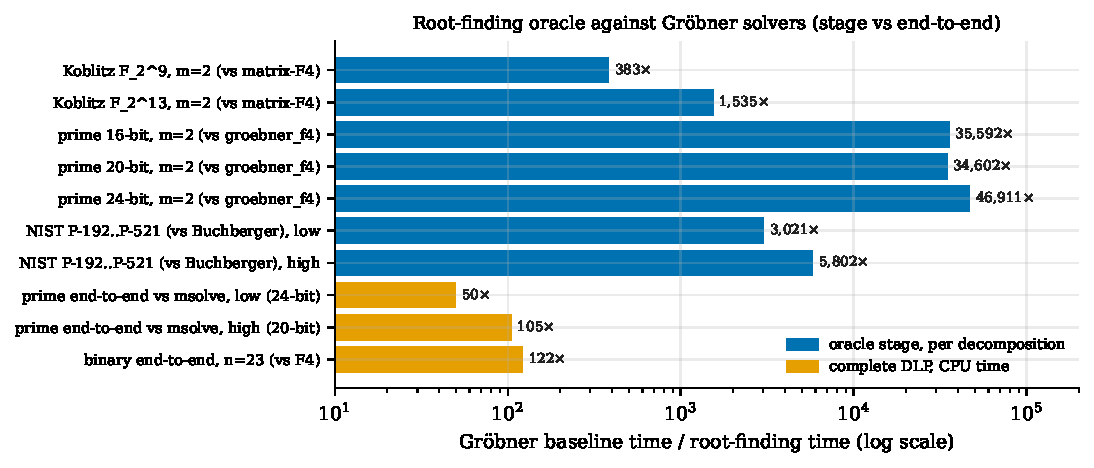
\includegraphics[width=\linewidth]{figures/fig-rootfind-oracle.pdf}
\caption[]{Root finding against Gr\"obner solvers on identical targets. Blue:
one decomposition (oracle stage only). Orange: complete discrete-log
computations with the oracle swapped and everything else fixed (prime: CPU
time against msolve, 20/24-bit totals composed from sampled per-query cost;
binary: one cold solve including table build). Sources:
\art{RESEARCH_SEMAEV_ROOTFIND_VS_GROEBNER.md},
\art{papers/rootfinding-decomposition/README.md}.}
\label{fig:rf-oracle}
\end{figure}

\paragraph{Oracle stage.} Per decomposition, root finding is
$383\times$ ($\FF_{2^9}$, $\abs\Fb=55$, 254 targets) and $1{,}535\times$
($\FF_{2^{13}}$, $\abs\Fb=4{,}005$, 256 targets) faster than matrix F4;
$3.5$--$4.7\cdot10^4\times$ faster than \texttt{groebner\_f4} on 16--24-bit
prime curves ($\abs\Fb=6$, 40 targets each); and $3{,}021$--$5{,}802\times$
faster than Buchberger on the decomposition ideal of the five NIST curves
(Figure~\ref{fig:rf-oracle}). Every binary verdict agreed with F4; every
prime solution was in F4's variety and every prime refutation was F4's unit
ideal. In the PDP study, \texttt{rf-mitm} refutes a binary target in
$3.1\,\mu$s at $\ell=8$ and $482\,\mu$s at $\ell=14$, against the PS-0
baseline's $9.3$\,ms and $55.5$\,s ($3{,}007$--$115{,}160\times$), costs
$5\abs\Fb-3$ multiplications and $2\abs\Fb$ lookups a target, and sits on
the pair-table floor at $1.000\pm0.027$ bits per rung; at prime $m=3$,
$N=18$ it uses 197 multiplications where F4 uses $8.99\cdot10^{13}$
multiply-adds; 707/707 brute-force agreements
(\art{research/pdp_root_finder_20261012/}).

\paragraph{Complete solves.} End to end, the gain is two orders of
magnitude smaller and not one-sided: $50$--$105\times$ against msolve on
16--24-bit prime curves; $122\times$ on the one binary instance ($n=23$)
large enough to amortise the pair table; and F4 \emph{faster} at
$n=5,9,13$, where a solve needs too few decompositions to pay for the
table. Inside ecbench, with every group operation charged, the
root-finding IC beats inherited F4 in solve wall by about $350\times$ at
$n=13$ (admitted) and about $10^4\times$ at $n=23$ (descriptive), yet stays
$2.9$--$25{,}116\times$ the strong rho in $S$ on binary curves and
$29$--$141\times$ rho on prime curves, with the gap widening
(\art{research/pdp_root_finder_ecbench_20261013/}).

\paragraph{The Koblitz loops.} Figure~\ref{fig:k13} follows the best
complete-count root-finding arm at Koblitz $E_0$, $n=13$ through four
registered improvement loops (8 public targets $\times$ 3 rounds each, L0
operation counts). The first engine had $S=38.82$ ($m=3$) and $28.38$
($m=2$). A windowed third-summand scan cut $m=3$ by a paired $0.828$
$[0.783,0.863]$; a fold over negation (\texttt{rootfind-negfold}) took
$m=2$ to $23.22$ and then $22.97$. Two further cycles of denser and
sparser bases, windowed negfold and plain root finding were dead ends
(\art{research/ecbench_rootfind_vs_rho_20261014/}). With F4's word XORs
priced, the paired ratio negfold/F4 is $0.0545$ $[0.047,0.064]$, a
complete-against-complete comparison; against strong signed-Frobenius rho
($S=14.82$) the best complete arm is still $1.55\times$. A compact-orbit
base with a counted Frobenius pair table reaches $S=15.55$, below the
then-unpriced F4 ($16.75$), but it is itself a lower bound
(factor-base construction natives unpriced), and it is $1.08\times$ rho.
Amortised over 64 targets that arm reaches $S\approx11.2$, below rho; by
the ledger's rules that is a secondary, multi-target result, not a cold
claim.

\begin{figure}[t]
\centering
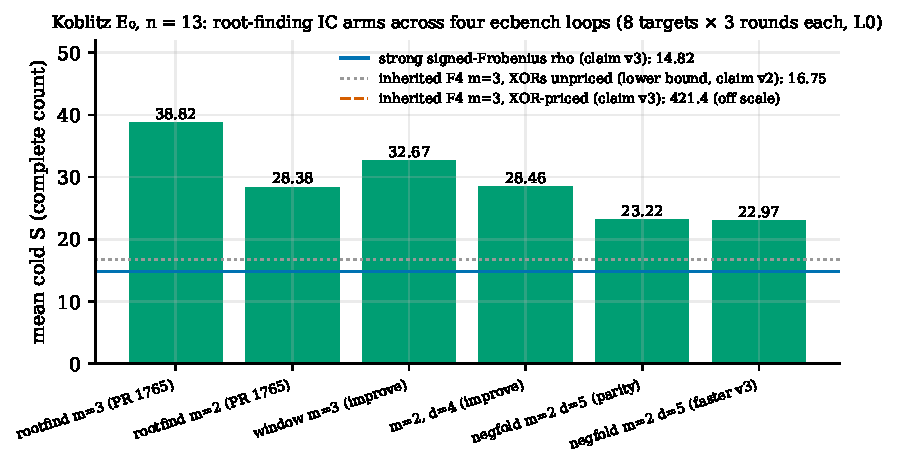
\includegraphics[width=\linewidth]{figures/fig-k13-progression.pdf}
\caption[]{Mean cold $S$ of root-finding IC arms at Koblitz $E_0$, $n=13$,
$d=5$ unless stated, across the engine, improve, parity and faster loops.
All bars are complete counts. Sources:
\art{research/ecbench_rootfind_engine_20261012/},
\art{research/ecbench_rootfind_improve_20261013/},
\art{research/ecbench_rootfind_parity_20261013/},
\art{research/ecbench_rootfind_faster_20261014/}. Each loop had its own
seeds and rho arm (rho $14.12$--$14.82$).}
\label{fig:k13}
\end{figure}

\paragraph{Prime tuning in ecbench.} On a 20-bit prime curve, the pair
table's counted $S$ is $0.018861$ $[0.018547,0.019242]$ of direct
subtraction (24 pairs; prime native work unpriced, so a bounded ratio), and
$0.057047$ $[0.041159,0.092069]$ on a 17-bit Koblitz curve, fully priced,
where the table set-up is about 68\% of the arm's cold cost. Doubling the
table from 32 to 64 abscissae gives $0.830$ $[0.697,0.962]$; three
summands instead of two costs $1.431\times$ $[1.225,1.716]$; batching the
table inversions leaves counted GAE unchanged ($1.000$; $4{,}096$ versus
$64$ inversions, set-up wall $243$ versus $128\,\mu$s, descriptive); and a
train-set lane selection did not resolve a hold-out winner ($0.979$
$[0.919,1.038]$; 1{,}088/1{,}088 verified executions)
(\art{benchmarks/README.md}, rows of 12--14 Oct).

\paragraph{Dense root index at $n=83$.} Widening the prefix base from
K1500 to K1798 cut mean probes per relation from $300{,}021.9$ to
$169{,}069.8$ (paired difference $130{,}952$, 95\% $[52{,}058,209{,}991]$)
and gave a one-point online ratio of $18.528$ over same-point rho (IC
$63.3$\,ms, rho $1{,}173.3$\,ms), with $339.0$\,s of reusable preparation
and an 8\,GiB table outside the window. The host was shared, so the result
is exploratory; two K1500 runs hit the 900\,s timeout and are retained.

\paragraph{Reading.} Root finding is the largest constant-factor change
of the programme at the oracle stage, and the one with a proof behind it.
It does not change the asymptotic count of index calculus: its cost is
$\Theta(\abs\Fb^{m-1})$, every measurement is at $m\le4$, and it leaves
relation yield, factor-base size and linear algebra untouched. Its effect
on the cold frontier is to move the decomposition stage from dominant to
minor, which exposes the stages that now are.

\section{Gr\"obner-basis engines}\label{sec:groebner}

Before root finding, the decomposition oracle was a Gr\"obner solve, and
for $m\ge3$ over binary fields it still is. The repository grew a family
of engines (\art{docs/ic/GROEBNER_F4F5F6_AUDIT_20261010.md}, \S1; file names below are under \art{src/cryptanalysis/}):

\begin{description}[style=nextline, leftmargin=1.4em]
\item[Matrix F4 and F5 over $\FF_2$] (\art{koblitz_groebner.rs},
  \art{matrix_f5_f2.rs}): Macaulay matrices of the Weil-restricted Boolean
  system, reduced by a shared Four-Russians kernel (\art{gf2_elim.rs}, four
  8-bit tables, AVX-512 or AVX2).
\item[Inherited F4] (\art{inherited_f4.rs}, from 22 September, the
  default algebraic oracle): a DPLL-style tree over partial assignments in
  which each child \emph{inherits} its parent's echelon form and re-reduces
  only what the assignment changed, instead of building a fresh Macaulay
  matrix per node.
\item[F6-IC] (opt-in): inherited F4 plus a factor-base domain gate (a
  fully assigned summand whose abscissa is not a base point refutes;
  partial support pruning refutes earlier), and meet-in-the-middle leaves
  (with $m-1$ summands fixed the last is looked up; at $m=3$ and
  $\abs\Fb\le256$ every compatible second point is added and the third
  looked up).
\item[$\FF_p$ F4] (\art{f4_fp.rs}, \art{f4_fp_tower.rs},
  \art{sig_fp_tower.rs}): degree-bounded F4 with sparse-by-reducer then
  dense reduction, a Faug\`ere--Lachartre block for the Kummer-tower
  oracle, and a signature variant.
\end{description}

\paragraph{Correctness.} The audit pinned every engine against every
other and against brute force (88+15+9+14+13+12+21+6 passing library
tests in the touched modules), and found one soundness bug
(\S\ref{sec:corrections}, item 6), two contract defects and several latent
holes, all fixed with regression tests.

\paragraph{Engineering results.} Figure~\ref{fig:engine} collects the
headline ratios; all are \cls{engineering} with identical outputs.
\begin{itemize}
\item \emph{Inherited versus matrix F4}: matrix work $198.6\times$ (K13)
  and $222.1\times$ (random-13) the inherited engine's on identical trees;
  at $m=19$ every matrix F4/F5 run timed out at 1{,}800\,s while
  inherited F4 finished in about 6\,s
  (\art{research/f4_f5_f6_cross_family_20261011/}).
\item \emph{F5 versus F4}: word-XOR ratios $0.6465$ / $0.6414$ (K13 /
  random-13), wall $0.79$--$0.86$.
\item \emph{F6-IC versus inherited F4}: word XORs about $0.82$ at $m=13$
  and $0.77$--$0.78$ at $m=19$, relation wall $1.7$--$1.9\times$ faster.
  But once its batched group additions are charged, F6-IC's $S$ is
  $64.6$--$68.8\times$ inherited F4's at $m=13$ and
  $1{,}303$--$1{,}353\times$ at $m=19$: an accounting loss, not a frontier
  move. At $m=31$ both engines hit the 3{,}600\,s cap on the first target.
\item \emph{Kernel routing and rewrite}: routing every echelon call to the
  Four-Russians kernel gave $1.75$--$3.22\times$ on the oracle's own
  Macaulay matrices; a word-level \texttt{pext}/\texttt{pdep} rewrite plan
  made F4 and F6-IC 10--14\% faster at $n=23$; eager rewrite of kept rows
  beat lazy rows by $1.40$--$1.62\times$
  (\art{research/inherited_f4_eager_rewrite_20261011/}).
\item \emph{Instruction and allocation work}, measured by paired A/B/A$'$
  instruction counts on a frozen eleven-system suite: fused construction
  and readback, $-5.28\%$ (F4) and $-11.02\%$ (F5) instructions; native
  hashing, $-3.715\%$ F5 $[3.714,3.726]$ and $-45.1\%$ for the standalone
  criterion; bounded direct indexing in the F5 packer, $-3.947\%$; row
  allocation, $42$--$50\%$ fewer requested bytes. Elapsed time was not
  claimed for these.
\item \emph{Quotient-curve model}: solving the $m=2$ system directly on
  the quotient curve instead of a symmetrised control cut F4 word
  operations by $1.340$--$1.642\times$ with identical root digests in five
  interleaved cells (\art{research/lit2026_w8_summation_models_20261011/}).
\item \emph{$\FF_p$ F4 to msolve parity}
  (\art{research/f4_fp_msolve_parity_20261011/}): Gebauer--M\"oller
  criteria, packed monomials, interned symbolic preprocessing and a
  parallel symbolic pass made \texttt{f4\_fp} $29.8$--$54.1\times$ faster
  than its predecessor on square generic systems, with msolve/ours at
  $0.96$--$1.22$ single-threaded. A day earlier msolve had been
  $12$--$24\times$ faster (\art{research/gb_cas_comparison_20261011/});
  every reduced basis agrees with Singular or msolve. On Boolean
  decomposition systems ($n=17$, 8 targets) our oracle decides in
  7--24\,ms per target, while msolve and PolyBoRi spend 40--52\,s computing
  a full basis and Singular exceeds 120\,s---a difference of task (decide
  versus compute the basis), not of engine quality.
\end{itemize}

\begin{figure}[t]
\centering
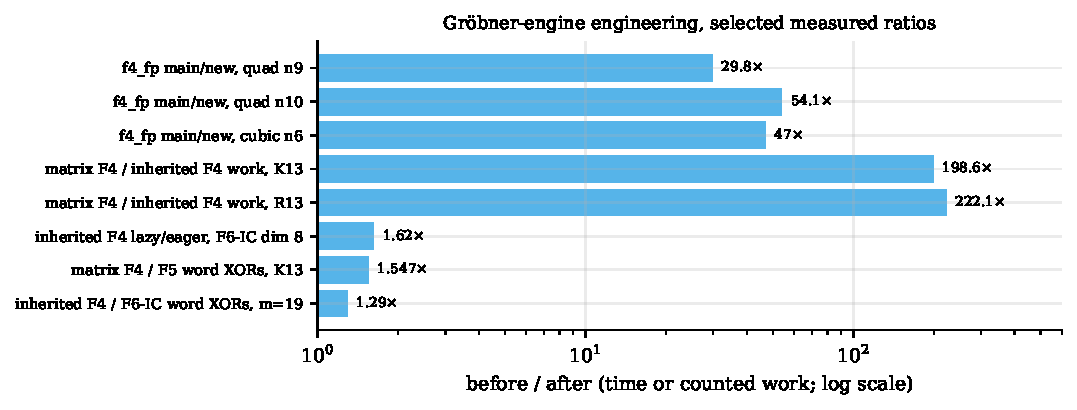
\includegraphics[width=\linewidth]{figures/fig-engine.pdf}
\caption[]{Selected engine ratios (before/after or baseline/candidate):
\texttt{f4\_fp} successive versions (single-threaded wall, L0); matrix
versus inherited F4 (counted matrix work); lazy versus eager inherited
rewrite (median wall); F4 versus F5 and inherited F4 versus F6-IC (word
XORs, stage only). Sources in \art{figures/data.json}.}
\label{fig:engine}
\end{figure}

\paragraph{What did not work.} Degree-2 early-abort probes after a
2025--26 proposal: word-XOR ratios $1.00083$--$1.00378$ (no change) and
$0.99714$--$0.99928$ (worse). Gate-first geometry: $1.57$--$1.78\times$
fewer word XORs but lane-batched F4 roots cost $2.6$--$4.0\times$ a
sequential control. Convolution splitting of the summation polynomial:
$1.21$--$2.07\times$ \emph{more} word operations despite lower degree;
Frobenius auxiliary variables: $57$--$701\times$ more
(\art{research/lit2026_w\{4,5,8\}_*_20261011/}). Symmetry-breaking clauses
in SAT did not help (\art{RESEARCH_KOBLITZ_INDEX_CALCULUS.md}). A
registered law for the $m=3$ refutation degree resolved all 68 units but
ended with the verdict ``neither'': one variant met its generic degree
window on 32/32 draws, the other fell below it on 8, and the heaviest
degree-10 Macaulay solves were $2.4\cdot10^5\times2.0\cdot10^5$ matrices at
42--51 minutes each (\art{research/ic_semiregular_law_20261005/}).

\section{Koblitz and binary curves}\label{sec:koblitz}

\subsection{Frobenius-invariant and compact-orbit bases}

The Koblitz implementation (\art{src/cryptanalysis/koblitz_index_calculus.rs})
builds GGMP's invariant base from the linearised polynomial of a factor of
$x^n-1$, checks $\pi(\Fb)=\Fb$ point by point, rewrites each relation into
orbit columns with known $\lambda^k$ weights, and solves the
cofactor-corrected system $h a+hbd\equiv\sum\lambda^{k_i}x_{o_i}$. On
small fields the orbit collapse is as predicted: $\abs\Fb/\#\text{orbits}$
of $7.86$, $10.89$, $12.96$ at $n=9,11,13$ for relations and
$61.7$--$168.0$ for linear algebra, against rho's $4.24$--$5.10$
(\art{RESEARCH_KOBLITZ_INDEX_CALCULUS.md}). Because $\ell=\operatorname{ord}_n(2)$
fixes the invariant base's size, the programme moved to bases sized to the
instance: divisor bases, SAT-optimised bases, a rank-guided base at $n=53$
(220 orbits, a complete implicit $\Sem5$ formula of 22{,}887 clauses), and
finally the \emph{compact signed-Frobenius orbit} base, which stores one
representative per orbit and no pair table
(\art{docs/ic/COMPACT_ORBIT_PRODUCER.md}). In the ecbench factor-base
suite it is the best measured Koblitz construction: $S=9.114$ at $n=17$
($272$ points, 8 columns), $9.985\times$ matched signed-Frobenius rho,
against full orbit $18.7\times$ and subspace bases $47\times$
(\art{research/ecbench_frontier_20261013/}).

\subsection{The oracle sequence}

The binary oracle went through SAT (XOR-native CDCL after Trimoska et
al.~\cite{trimoska2020}; decides the $n=19$, $\ell=6$ corpus but does not
scale), matrix F4 (whose refutation range was the real frontier),
pairs-and-solve for $\Sem4$ (validated to $n=21$, $\ell=7$, still
$O(2^{2\ell})$), meet-in-the-middle pair tables, inherited F4 and F6-IC
(\S\ref{sec:groebner}), and root-finding engines (\S\ref{sec:rootfinding}).
The boundary ledger's current Koblitz decomposition record is an $n=31$,
$m=2$ F4 cell with an exact block-6 M4RI acceleration; at $n=53$ an exact
Frobenius-orbit $\Sem5$ compression removes the coordinate ROM but every
unrestricted solver arm remains \textsc{unknown}.

\subsection{The one-target online ladder}

The ledger's primary \texttt{vs\_rho} question is: with reusable IC
preparation already done, how long does one unseen public target take,
against rho with the automorphism discount on the same point? The ladder
(Figure~\ref{fig:online}):

\begin{itemize}
\item $n=53$: guided shared-log precompute with an explicit pair table
  (9.34\,GB peak RSS); earlier, a 1{,}024-target shared-log batch beat
  batched rho in all 15 paired blocks (secondary, multi-target).
\item $n=61$: compact orbit, 600 columns, 73{,}200 points, 2.73\,GB; fresh
  reproduction $124.85\times$ (exploratory).
\item $n=71$: first rung past 64-bit packing (u128 words), 85{,}200
  points, $2{,}864.1\times$ median of three repeats of one point
  (exploratory).
\item $n=73$: 87{,}600 points, $1{,}189.7\times$; the guided-rank
  precompute took 5.1\,h at 57--70 million probes per relation
  (exploratory).
\item $n=83$, $a=1$: IC online 5.6--7.9\,s against rho 43--71\,s,
  $8.2\times$; then the dense root index, $18.5\times$ (both exploratory).
\item \textbf{$n=61$, admitted} (12 October): $a=0$, $K=500$ orbit
  columns, $61{,}000$ points, 64 fresh public one-target workloads per
  host, identical candidate manifest on two hosts. Pinned x86\_64:
  median online speed-up $13.94\times$, 95\% $[9.81,19.13]$, claim-check
  64/64; unpinned arm64: $12.87\times$ $[7.30,19.08]$. Set-up of about
  28\,s is outside the window; with it charged, IC costs a median
  $83.4\times$ rho.
\end{itemize}

\begin{figure}[t]
\centering
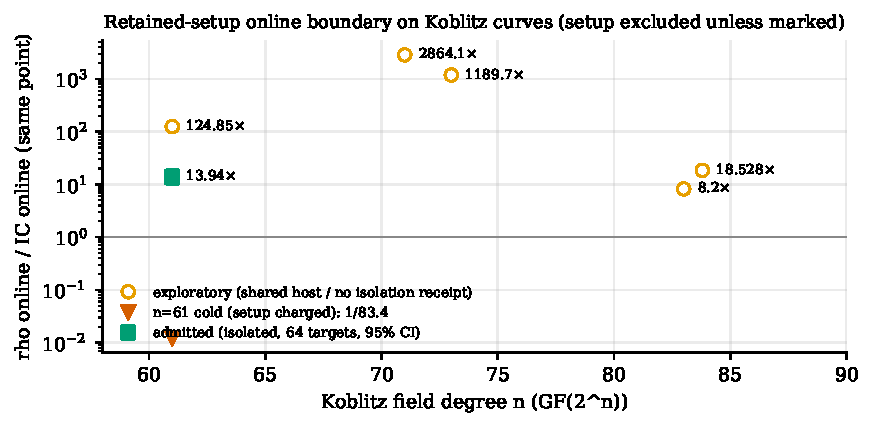
\includegraphics[width=\linewidth]{figures/fig-koblitz-online.pdf}
\caption[]{Rho online time over IC online time on the identical public point,
reusable IC preparation excluded. Open circles: exploratory (verified
answers, no qualifying isolation receipt; three repeats of one point or a
single point). Filled square: the admitted 64-workload panel with its 95\%
bootstrap interval. Triangle: the same $n=61$ candidate with set-up
charged (cold). Sources: \art{docs/ic/boundary_targets.json},
\art{docs/ic/PLAN_IC_ACCOUNTING_FIXES_20261007.md},
\art{research/n83_dense_root_20261013/}.}
\label{fig:online}
\end{figure}

The exploratory ratios are large and irregular because a one-point online
window measures the luck of one relation search against one rho walk; the
admitted panel's range over 64 workloads is $1.06$--$648.6\times$. The
admitted point is a constant-factor online result at $n=61$ (47-bit
subgroup) with preparation retained; it is not a cold result, not a
scaling law, and not an asymptotic claim. By the frontier's own arithmetic
the $n=83$ preparation would pay for itself after $q^*=306$ targets
(derived what-if: reusable set-up $339.0$\,s, online $0.0633$ versus
$1.173$\,s; assumes constant per-target cost and zero rho set-up).

\emph{Retired as an index-calculus win (14 October).} Every rung of this
ladder compares index calculus with a retained table against rho with
none. Given a distinguished-point table of equal or smaller size,
Bernstein--Lange preprocessing rho~\cite{bl2012} is $53$--$317\times$
faster online than the compact-orbit arm on the same 64 targets at $n=41$,
53 and 61 (\S\ref{sec:ladder}). The ladder therefore measures what a
table buys, and generic rho buys more per byte.

\subsection{ECC2K-130}\label{sec:ecc2k130}

ECC2K-130 is the $a=0$, $n=131$ member of the same family; the compact
producer already solves $n=41,53,61,71,73$ of it. Extrapolating the fitted
probes-per-relation law $C\,r/(n^2K^2)$ with $C=1$ gives
$1.1\cdot10^{18}$ core-years at $K=600$ and $6.8\cdot10^{8}$ at
$K=10^{12}$ columns (\art{RESEARCH_ECC2K130_IC_FEASIBILITY.md}, with the
unexplained factor-of-5 gap in $C$ of \S\ref{sec:corrections}). The
separate GPU rho estimate for the same curve is about 4.3 RTX PRO 6000
card-years (\art{paper/ecc2k130/}). Index calculus is not a route to
ECC2K-130 on this evidence; the isogeny-class routes are discussed in
\S\ref{sec:transfer}.

\section{Prime and extension fields}\label{sec:prime}

\subsection{Known-answer ladders over $\FF_p$}

Over prime fields the ledger tracks staged known-answer ladders
(\art{docs/ic/boundary_targets.json}, regime \texttt{prime}). On $j=0$
curves the staged driver recovers a 20-bit logarithm
($p=1{,}048{,}609$) in 56.8--64.9\,s of IC wall against 150--153\,ms of rho
on the identical public point, with split timers and three seeds. On the
generic $a=-3$ shape (P-256 and CryptoPro-B class), a Semaev-$\Sem4$
three-decomposition family with Cantor--Zassenhaus root finding yields one
relation per trial at $p=65{,}519$ with a 120-point base; at fixed base
size, median trials per relation grow from 2 to 28 to 379--506 at 16, 20
and 24 bits, about $16\times$ per four bits. The prime \texttt{vs\_rho}
row is \emph{not achieved} at any measured size.

\subsection{PDP oracle programme}

The point-decomposition (PDP) speed-up programme
(\art{research/pdp_oracle_speedup_20261011/}) measured the oracle in three
steps before root finding replaced it: a baseline (PS-0; $338$--$452$\,ns
per pair across five rungs, A/A spread $\le8.8\%$), a gate-count model of
the group-law form (PS-1; $7{,}410$--$14{,}608$ fused ternary-logic issues
against $70{,}695$--$190{,}275$ for the derived baseline, $9.5$--$13.0\times$),
and a scalar group-law kernel (PS-2; $29.8$--$40.8$\,ns per pair, per-pair
ratio to baseline $0.067$--$0.123$, 400 corpus root sets agreeing). A
split/hybrid solving-degree study then projected its closest relation phase
at $22.8\times$ strong rho (\art{research/pdp_split_dreg_20261011/}), with
an initial read-out defect preserved in the record.

\subsection{Kummer-tower factor bases}

Petit, Kosters and Messeng's base $V=\mu_{2^t}$ (the roots of
$x^{2^t}-1$) gives prime-field summation systems extra structure for an
algebraic solver. We ran it end to end in ecbench with the root-finding
oracles on five curves of 20--28 bits (896 runs, all verified, all replay
audits OK; \art{research/pkm_tower_ecbench_20261013/}). Index calculus
costs $34.0$, $41.9$, $29.4$, $96.6$ and $140.6\times$ rho-negation in $S$
(95\% intervals in Figure~\ref{fig:prime}), growing by $0.26\pm0.28$ bits of
$S_{IC}/S_\rho$ per bit of $r$, consistent with the $p^{1/6}$ the floors
predict. The tower base costs the same as a plain base of the same size to
within 1\% (ratios $0.999$--$1.012$): PKM's structure helps an algebraic
solver, not a table.

\subsection{Gaudry's $k=4$ index calculus over $\FF_{p^4}$}\label{sec:gaudry}

Over $\FF_{p^k}$ with a base of points whose abscissa lies in $\FF_p$, a
relation needs a $k$-decomposition solved by a Macaulay system. We made the
\texttt{gaudry\_quartic} solve generic in the number of unknowns and faster
(median whole solve $1.9$/$4.1$/$6.4\times$ at $d=4,5,6$, $37.4\to5.9$\,s
at $d=6$; the $\Sem5$ solve from about 30 minutes to 164--203\,s; every
count and solution identical). Then we built FGHR's $D_4$ variant
(\art{research/gaudry_quartic_d4_20261013/}): on a curve with rational
2-torsion $T$, the coordinate $Y=(x-x_0-c)/(x-x_0+c)$ satisfies
$Y(P+T)=-Y(P)$, so $\Sem5$ in $Y$ is invariant under the Weyl group $D_4$
(order 192). In the invariants $\sigma_k=e_k(Y^2)$, $\pi=\prod Y_i$, the
system has B\'ezout number 512 instead of 4{,}096, Macaulay degree 14
instead of 29, and a $13{,}412\times11{,}628$ matrix instead of
$41{,}780\times40{,}920$.

At $p=269$, the cost $C_4$ of one decomposition falls from
$1.21$--$1.23\cdot10^{12}$ to $2.54$--$2.55\cdot10^{10}$ $\FF_p$
multiplications, $47.5$--$48.4\times$; a solve takes 4.2--5.6\,s instead of
164--203\,s. Decompositions agree with an independent meet-in-the-middle
enumeration on 19 of 19 solved targets; one target in 20 is degenerate
(quotient dimension 517) and is discarded, adding about 5\% to the
relation phase. The $Y$-line base decomposes about $1/8$ as often (pooled
ratio $0.133$ over 8{,}000 targets; prediction $1/8\pm30\%$ held on one of
two curves), but each column covers $\{\pm P,\pm(P+T)\}$, halving the
unknowns.

Inserted into the repository's crossover model
(\art{research/notes/index-calculus/RESEARCH_RESIDUAL_WALKS.md} \S11.16), the measured $C_4$ and rate move
the $k=4$ crossover with rho from $2^{149.4}$--$2^{152.7}$ to
$2^{135.1}$--$2^{135.8}$ (cofactor $h=2$, forced by the 2-torsion), and
the asymptotic ratio past it from $0.34$--$0.63$ to $0.12$--$0.22$ of rho.
This is the one place in the programme where a crossover moves; it moves
in an \emph{extrapolated model} ($n^{1/4}$ relations, $n^{1/2}$ linear
algebra and rho) fed by a measured constant, so it is classed as
\cls{engineering}, not an advance. Extension fields of degree four are not
the fields deployed curves use.

\begin{figure}[t]
\centering
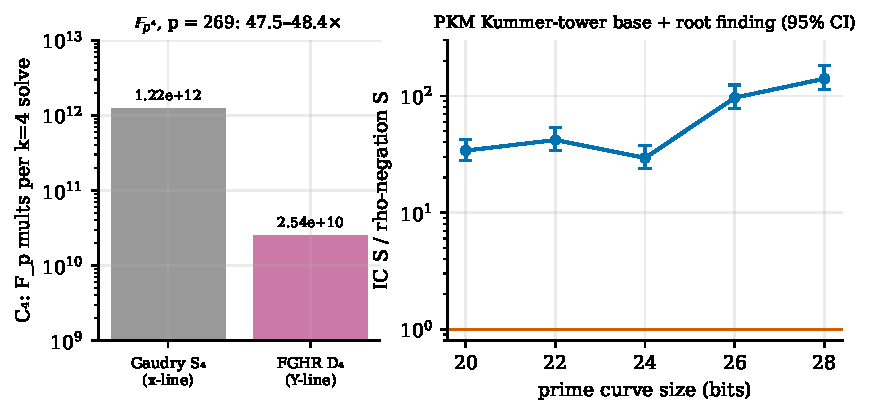
\includegraphics[width=\linewidth]{figures/fig-prime.pdf}
\caption[]{Left: cost $C_4$ of one $k=4$ decomposition over $\FF_{p^4}$,
$p=269$, Gaudry's $S_4$ system on the $x$-line against FGHR's $D_4$ system
on the $Y$-line (\art{research/gaudry_quartic_d4_20261013/}). Right:
index calculus with the PKM tower base and root finding over rho with
negation, eight one-target workloads $\times$ three rounds per size,
paired 95\% cluster-bootstrap intervals
(\art{research/pkm_tower_ecbench_20261013/}).}
\label{fig:prime}
\end{figure}

\subsection{Literature claims that did not survive}

The lit2026 programme (\art{research/lit2026_speedup_program/}) ran each
finding of a 2025--26 search as a measured change against an interleaved
baseline binary. Workstream W12 implemented the zero-minor
guess-and-determine attack (Mahalanobis, arXiv~2607.09814v2): it solved
48/48 planted targets on 16--26-bit curves, but its search phases scale
with slope $0.905$ $[0.769,1.021]$ in $\log_2 r$ and its cost over rho
grows from $260\times$ to $6{,}715\times$---exhaustive in $r$, as the
source's own table says. A second flagged ePrint (Hu, 2025/015) did not
specify an implementable algorithm and is recorded as blocked. On the
generic side, W11 cut BSGS from $16.75$ to $3.71$ multiplication
equivalents per visited point with paired steps (wall $1.15$--$1.67\times$),
which moves rho's and BSGS's constants, not index calculus.

\section{Isogeny, transfer and structure routes}\label{sec:transfer}

A recurring hope was that some other representation of the same
instance---an isogenous curve, a curve at another level of the isogeny
volcano, a Jacobian, a Weil descent---would make index calculus cheaper.
These routes produced the programme's clearest negatives, and one lemma
that explains most of them.

\begin{lemma}[transport conservation,
\art{docs/ic/RESEARCH_TRANSFER_AWARE_IC_20261010.md} \S1]\label{lem:conservation}
Let $\varphi:E\to E'$ be an $\FF_q$-rational isogeny (or any homomorphism
of rational points), $\kappa=\ker\varphi\cap E(\FF_q)$, $R\in E(\FF_q)$,
$\Fb'\subset\varphi(E(\FF_q))$ a factor base on the codomain and
$\Fb=\varphi^{-1}(\Fb')\cap E(\FF_q)$. Then the number of ordered
$m$-decompositions of $R$ over $\Fb$ is $\abs\kappa^{m-1}$ times the number
of ordered $m$-decompositions of $\varphi(R)$ over $\Fb'$.
\end{lemma}
\begin{proof}
Images of decompositions of $R$ are decompositions of $\varphi(R)$.
Conversely, for $\sum Q_i=\varphi(R)$ choose rational preimages $P_i$ of
the $Q_i$; then $\sum P_i-R\in\kappa$, and of the $\abs\kappa^m$ choices
exactly $\abs\kappa^{m-1}$ sum to $R$ (translate $P_1$ by the kernel
element).
\end{proof}

So a homomorphic transfer changes nothing but three curve-specific inputs:
the rational kernel symmetry $\abs\kappa^{m-1}$ (bounded by the rational
torsion; trivial on prime-order curves), the factor-base geometry
available on the destination, and the cost of arithmetic there. Sequences
of isogenies compose to one homomorphism; a loop is an endomorphism and
acts on the subgroup as a known scalar, useful only as a known-log
multiplier. Multi-curve factor bases glued by isogenies are single-curve
bases in disguise.

\paragraph{Conductor gaps in the ECC2K-130 class.} Jao, Miller and
Venkatesan~\cite{jmv2005} prove random self-reducibility among curves with
the same endomorphism ring, leaving open whether curves whose conductors
differ by a large prime could differ in hardness. The ECC2K-130 class has
conductor gap 263; we computed its structure
(\art{docs/ic/RESEARCH_ISOGENY_CONDUCTOR_GAP_20261007.md}) and ran
several rounds of experiments. Native counted-$S$ index calculus on two fixed CM
pairs gave floor/crater ratios $0.975$ (99\% $[0.603,1.451]$) at
$\ell=8209$ and $1.127$ $[0.922,1.342]$ at $\ell=131101$: no level effect
(192 verified records, 96 exact replays;
\art{research/ecbench_conductor_gap_20261012/}). Two-torsion
symmetrisation is a quotient isogeny: at a matched base of abscissae it
cut F4 row-reduction work $4.1$--$4.3\times$ ($\abs H=2$) and
$17.6$--$19.6\times$ ($\abs H=4$) over 1{,}128 systems---but a correction
the next day showed that at a matched number of \emph{columns} the saving
disappears; it was the cost of a redundant orbit base. A combined Weil
descent used $234$--$529\times$ the F4 operations of the blind system
(\art{research/isogeny_conductor_gap_round3_20261011/}).

\paragraph{Fibre-aware index calculus.} Isogeny fibres are torsors whose
arithmetic is controlled by one cohomology class
(\art{RESEARCH_ISOGENY_FIBERS_ECDLP.md}); relation generation is
isogeny-equivariant at zero lifting cost, and a fibre-closed pair table was
the best lever of the conductor-gap rounds ($12.8\times$ rho in its best
cell). Measured against matched rho across sizes at fixed cofactor, the
envelope IC/rho ratio grows from $8.4$--$8.8$ to $35.1$--$37.0$ ($h=4$) and
from $13.4$--$20.1$ to $60.4$--$63.1$ ($h=72$), as $\#E^{1/6}$: the gap
widens, it does not close (816 audited records;
\art{research/fiber_ic_scaling_20261011/}).

\paragraph{Other structure.} Symmetrised $u$-frame bases saved
$0.84\times$ at $n=17$ and $0.76$--$0.77\times$ at $n=23$, but cost
$4.01\times$ at $n=31$ (\art{research/koblitz_symmetrised_e2e_20260927/}).
GHS and hyperelliptic covers: ECC2K-130 does map to hyperelliptic curves,
but the genus that would pay is missing. In odd characteristic the cubic
GHS transfer from $E_0(\FF_{q^3})$ to a genus-3 Jacobian now runs end to end
with double-large-prime index calculus, at $q^{1.380}$ against rho's
$q^{3/2}$, still $1.7$--$2.6\times$ the negation-map rho model at
$q=2^{20}$ (\S\ref{sec:ladder}). The
isogeny-loop GLV/GLS work produced a measured $1.09$--$1.15\times$ faster
four-dimensional scalar multiplication (\art{research/isogeny_loop_glv_20261012/})
and a $\sqrt{\text{\'elu}}$ kernel cost exponent $0.822$ $[0.805,0.838]$;
these speed up curve arithmetic, not the discrete logarithm.

\paragraph{Named obstructions.} Blocked requirements are kept open as
problem records (\art{problems/README.md}), among them the complete-cost
calibration of root-finding IC
(\art{problems/rootfinding-complete-cost-calibration.md}), with exit
criteria rather than abandoned.

\section{What improved, and where the frontier stands}\label{sec:frontier}

Table~\ref{tab:improvements} collects the measured improvements of the
programme on the boundary each was measured on. Ratios are
baseline/candidate; ``stage'' means one oracle call or one solver run;
``complete'' means a verified discrete logarithm with the stated phases.

\begin{table}[p]
\centering\small
\caption[]{Measured improvements, July--October 2026. Class: E =
\cls{engineering}, A = \cls{accounting}. Boundary: St = stage,
Cx = complete solve outside ecbench, Cold = ecbench cold one-target $S$,
On = online window after retained set-up. Sources: Appendix~\ref{app:artefacts}.}
\label{tab:improvements}
\begin{tabularx}{\linewidth}{@{}>{\raggedright}Xllr>{\raggedright\arraybackslash}p{3.0cm}@{}}
\toprule
Change & Bnd. & Cl. & Ratio & Scope \\
\midrule
\multicolumn{5}{@{}l}{\emph{Decomposition oracle: root finding}}\\
$\Sem3$ roots, binary pair table vs matrix F4 & St & E & $383$--$1{,}535$ & $\FF_{2^9}$, $\FF_{2^{13}}$, $m=2$ \\
$\Sem3$ roots, prime vs \texttt{groebner\_f4} & St & E & $3.5$--$4.7{\cdot}10^4$ & 16--24-bit, $\abs\Fb=6$ \\
$\Sem3$ roots vs Buchberger, NIST curves & St & E & $3{,}021$--$5{,}802$ & P-192\ldots P-521 \\
\texttt{rf-mitm} vs PS-0 oracle & St & E & $3{,}007$--$115{,}160$ & binary $\ell=8..14$ \\
Root-finding DLP vs msolve DLP & Cx & E & $50$--$105$ & 16--24-bit prime \\
Pair-table DLP vs F4 DLP & Cx & E & $122$ & binary $n=23$ (F4 wins $n\le13$) \\
Pair table vs subtraction & Cold & E & $53.0$ & 20-bit prime (bounded) \\
Frobenius pair table vs subtraction & Cold & E & $17.5$ & Koblitz $n=17$, priced \\
Root-finding K13 arm, first to best & Cold & E & $1.69$ & $38.82\to22.97$, across sessions \\
Windowed $m=3$ scan & Cold & E & $1.21$ & $[1.16,1.28]$ \\
Negfold root finding vs XOR-priced F4 & Cold & E & $18.3$ & $[15.6,21.3]$, K13 \\
Dense root index K1798 vs K1500 (probes) & On & E & $1.77$ & $n=83$, one point \\
Pair-table size 64 vs 32 abscissae & Cold & E & $1.20$ & $[1.04,1.43]$ \\
\addlinespace
\multicolumn{5}{@{}l}{\emph{Gr\"obner engines}}\\
Inherited vs matrix F4 (matrix work) & St & E & $198.6$--$222.1$ & K13, R13 \\
F5 vs matrix F4 (word XORs) & St & E & $1.55$--$1.56$ & K13, R13 \\
F6-IC vs inherited F4 (word XORs) & St & E & $1.22$--$1.30$ & $m=13,19$ \\
\texttt{f4\_fp} new vs previous & St & E & $29.8$--$54.1$ & square systems, = msolve \\
Four-Russians routing & St & E & $1.75$--$3.22$ & oracle matrices \\
Eager vs lazy inherited rewrite & St & E & $1.40$--$1.62$ & dim 8--9 \\
Quotient-curve $m=2$ model & St & E & $1.34$--$1.64$ & five cells \\
\addlinespace
\multicolumn{5}{@{}l}{\emph{Factor bases and symmetry}}\\
Compact orbit vs full orbit & Cold & E & $\le1.87$ & Koblitz $n=17$; compact is LB \\
FGHR $D_4$ vs Gaudry $S_4$, $C_4$ & St & E & $47.5$--$48.4$ & $\FF_{269^4}$ \\
\texttt{gaudry\_quartic} solve & St & E & $1.9$--$6.4$ & $d=4..6$ \\
\addlinespace
\multicolumn{5}{@{}l}{\emph{One-target online}}\\
Compact-orbit IC vs strong rho & On & E & $13.94$ & $n=61$, $[9.81,19.13]$, 64 targets \\
\addlinespace
\multicolumn{5}{@{}l}{\emph{Accounting (costs that went up when priced)}}\\
F4 word XORs priced & Cold & A & $1/25.2$ & $16.75\to421.4$, K13 \\
F6-IC batched geometry priced & Cold & A & $1/64.6$--$1/1{,}353$ & $m=13,19$ \\
\bottomrule
\end{tabularx}
\end{table}

\noindent Derived entries: $53.0=1/0.018861$; $17.5=1/0.057047$;
$1.21=1/0.828$ with interval from $[0.783,0.863]$; $18.3=1/0.0545$ with
interval from $[0.047,0.064]$; $1.77=300{,}021.9/169{,}069.8$; $1.20=1/0.830$
with interval from $[0.697,0.962]$; $1.87=18.714/9.985$ (one session; the compact arm's $S$ is a lower bound, so
the ratio is an upper bound); $1.69$ and $25.2$ compare means from different
sessions with different seeds and are descriptive; F5 and F6-IC ratios are
reciprocals of the recorded candidate/baseline word-XOR ratios.

\subsection{Three frontiers}

\paragraph{Cold, one target, set-up included.} Unchanged: generic rho.
Every measured index-calculus arm is above its matched rho
(Figure~\ref{fig:cold}); the closest complete count is root-finding negfold
at $1.55\times$ strong signed-Frobenius rho at $n=13$; the closest
lower-bound arms are $1.08\times$ (compact orbit with a counted Frobenius
table) and $6.97\times$ (matrix F4/F5 against rho-negation at K13).
Prime-field arms are $12$--$239\times$ rho and diverge with size.

\paragraph{Online, after retained set-up.} One admitted point: compact-orbit
IC at Koblitz $n=61$, $13.9\times$ $[9.8,19.1]$ over strong rho on 64
unseen public targets, set-up of about 28\,s excluded (cold median
$83.4\times$ rho). The larger $n=71,73,83$ observations remain exploratory.

\paragraph{Stage.} Moved substantially: the decomposition oracle is two to
five orders of magnitude cheaper than at the start of the programme on the
workloads where root finding applies, the $\FF_p$ F4 is at msolve parity,
the Boolean F4 family is one to two orders of magnitude cheaper in counted
matrix work, and the $k=4$ extension-field solve is $48\times$ cheaper.
None of this, by itself, moves the cold frontier: the stages it leaves
untouched---relation yield, factor-base size, linear algebra, table
set-up---now dominate.

\begin{figure}[t]
\centering
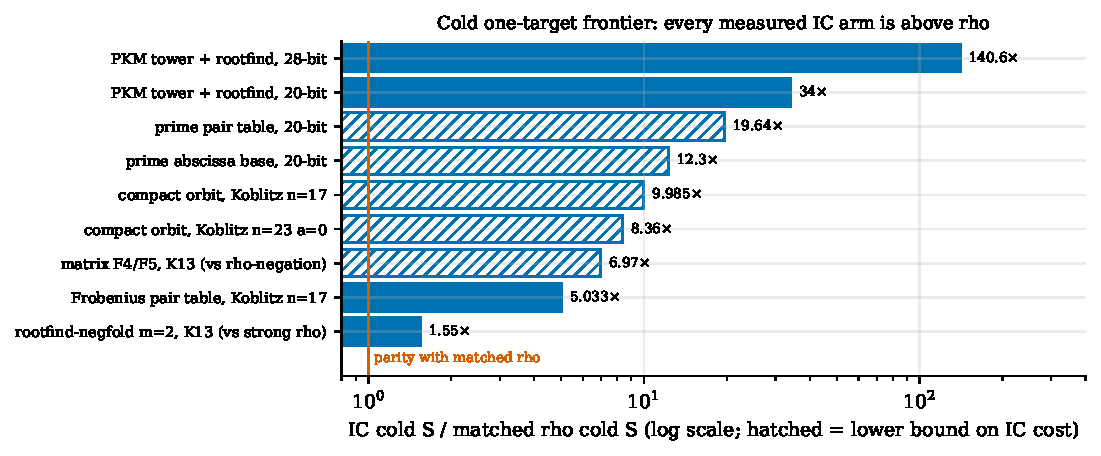
\includegraphics[width=\linewidth]{figures/fig-cold-gap.pdf}
\caption[]{Cold one-target $S$ of index-calculus candidates over their
matched rho arm (each study's own estimator; curves differ, so bars are not
ranked against each other). Hatched: lower bound on IC cost (unpriced
native or solver work). Sources: \art{research/ecbench_frontier_20261013/},
\art{research/ecbench_rootfinding_assessment_20261012/},
\art{research/pkm_tower_ecbench_20261013/},
\art{research/ecbench_rootfind_faster_20261014/}.}
\label{fig:cold}
\end{figure}

\subsection{What would move the cold frontier}

From the frontier synthesis and the problem records: (i) register the
torsion-symmetrised bases and the $n=83$ dense-root engine in ecbench under
immutable method identities and emit cold and online records; (ii) resolve
the inherited-F4 cross-host counter drift before using that counter in a
bound; (iii) run a four-size native challenge against the standing rho
bound---two sizes cannot establish an exponent; (iv) obtain an isolated
cold session at $n=83$ with every set-up phase and retained byte charged;
(v) price F6-IC's batched geometry with a pinned conversion. A result in
the cold domain that beats rho at four sizes would be the first
\cls{advance} of the programme.

\section{Open problems and proposed experiments}\label{sec:open}

% Survey section (draft 2026-10-15). Each problem is phrased as the
% measurement or proof that would settle it, per the repository's
% "name the obstruction" rule.

\paragraph{1. The solving degree of Weil-descended summation systems.}
Every subexponential claim for prime-degree binary curves rests on a bound
for this degree (\S\ref{sec:theory}); none is proved and the experimental
evidence is contested. \emph{Experiment:} measure first-fall, last-fall
and solving degree of $\Sem{m+1}$ restricted to $\ell$-dimensional
subspaces over a grid of $(n,\ell,m)$ with $m\ge3$, at least four values
of $n$ per $(\ell,m)$, against the semi-regular prediction, with
multi-graded regularity (one block per summand) as a second model.
\emph{Settles:} whether the degree grows with $n$ at fixed $(\ell,m)$; a
growth consistent with zero would revive the Petit--Quisquater and Semaev
heuristics, a positive slope would close them for this model.

\paragraph{2. Cold index calculus against rho with every operation
priced.} No measured arm beats matched rho on the cold one-target boundary
once native work is priced on both sides (\S\ref{sec:frontier}).
\emph{Experiment:} the frontier campaign of \S\ref{sec:frontier} extended
to the largest sizes each arm can reach, with exponents fitted per arm and
the crossover reported only where the fitted exponents separate across the
whole pricing band. \emph{Settles:} whether any implemented arm has an
exponent below $1/2$ in $r$ on these families.

\paragraph{3. Relation yield is now the dominant stage.} Root finding made
the decomposition oracle cheap; what remains is the number of trials per
relation, governed by the factor-base density. \emph{Experiment:} for each
factor-base family, the measured trials-per-relation law against $r$ and
base size, compared with the counting prediction $m!\,r/N^{m-1}$; the
residual (e.g.\ the unexplained factor 5 in the ECC2K-130 extrapolation,
\S\ref{sec:koblitz}) is the target.

\paragraph{4. Root finding beyond two summands on prime curves.} The
two-summand oracle is prior art in mechanism (McGuire--Mueller) and costs
$\Theta(N)$ per trial; three summands cost a pair table of $N^2$ entries.
\emph{Question:} is there a sub-$N^2$ structure for $\Sem4$ membership
over a prime-field base---for example from the $D_m$-invariant coordinates
of 2-torsion curves---and does it change the $r^{2/3}$ cost of two-summand
prime index calculus? A negative answer with a counting argument would be
as useful as a positive one.

\paragraph{5. The preprocessing regime.} Index calculus with a retained
table beats rho without one, and loses by $53$--$317\times$ to
Bernstein--Lange rho with an equal or smaller table (\S\ref{sec:ladder}).
\emph{Experiment:} measure the advice--time curve $(S,T)$ of the
compact-orbit arm across sizes against preprocessing rho's
$S\,T^2\approx N$; an index-calculus online result counts only if it lies
below that curve at equal $S$.

\paragraph{6. Symmetry at $k=4$, end to end.} The $D_4$ reduction and its
four-unknown weighted form move a \emph{modelled} handover over $\FF_{p^4}$
from about $2^{150}$ to $2^{119}$--$2^{137}$ depending on frame
(\S\ref{sec:ladder}).
\emph{Experiment:} a complete $k=4$ index calculus over $\FF_{p^4}$ at
several $p$, cold, priced, against rho with the available automorphisms,
to replace the model by a measured slope.

\paragraph{7. Pricing and calibration infrastructure.} Rankings now
require every arm's native work to be counted (AGENTS.md \S5a).
\emph{Work:} count the three uncounted categories of the shared-rank arm;
calibrate every ladder size on one fixed host; resolve the inherited-F4
cross-host counter drift; register the $n=83$ dense root index in the
harness.

\paragraph{8. Genus three after cubic GHS, to the crossover.} The one
family whose fitted exponent ($q^{1.380}$) lies below rho's $q^{3/2}$ is
still $1.7$--$2.6\times$ the negation-map rho model at $q=2^{20}$, and its
local exponent rises by $0.02$ per bit because the linear algebra grows as
$q^{1.5}$ (\S\ref{sec:ladder}).
\emph{Experiment:} rebalance the factor-base fraction to the structured
linear algebra, price a multiplication mod $\ell$ at its measured cost, and
run to $q\ge2^{22}$ against a measured negation-map rho on the same
instances, in the harness and across the pricing band. A measured
crossover there would be the programme's first \cls{advance} against rho,
on a narrow and undeployed family.

\section{Conclusion}\label{sec:conclusion}

Fourteen weeks of work produced three kinds of result. The first is
infrastructure: a single unit and harness in which rho, BSGS, the kangaroo
and every index-calculus variant are charged the same way on the same
one-target workloads, with sealed records, exact replays and admitted
intervals; and a ledger that refuses a claim with a missing field. The
second is a set of constant-factor improvements, the largest of which---the
closed-form roots of $\Sem3$---began as one sentence in a manuscript we were
asked to check, and ended as a proved identity, an oracle family covering
prime and binary fields, two to four summands, CPU and GPU, plain, tower
and dense-index bases, and the default decomposition strategy of the
codebase. The third is a map of what does not work, which is longer than
the list of what does: SAT that does not scale, symmetry that pays at
$n=17$ and costs at $n=31$, transfers that provably cannot change
decomposition counts, fibre-aware bases whose gap to rho grows as
$\#E^{1/6}$, literature attacks that are exhaustive search.

The honest summary is the campaign of \S\ref{sec:campaign}. On the
question the survey asks---does index calculus solve one unseen
elliptic-curve target, cold, for less than rho?---the answer on every curve
we measured, at every weight of the pricing band, is no. The closest arm is
a compact Frobenius-orbit Koblitz index calculus at $4$--$18\times$
signed-Frobenius rho, prime-field index calculus falls behind as $r^{1/6}$,
and no fitted exponent of an index-calculus arm lies below rho's. The
online $13.9\times$ at $n=61$ compared a table against no table and loses
$53$--$317\times$ to preprocessing rho with equal advice; it is retired.

Measured against its own baseline, which is the criterion the programme now
works to, index calculus keeps improving: about twenty changes landed on
14--15 October, among them a genus-3 index calculus after cubic GHS
whose exponent (about $q^{1.4}$) lies below rho's $q^{3/2}$, an $18\times$ cheaper
$k=4$ ladder and a further $18\times$ cheaper $k=4$ solve, and production
free relations on Koblitz curves ($0.960\times$). The genus-3 family is
the nearest to rho: $1.15\times$ a measured negation-map rho at $q=2^{20}$
after the second round, with a further $0.62\times$ step not yet matched
against rho. The stages that now
dominate are relation yield, factor-base size and linear algebra, and the
open problems of \S\ref{sec:open} say what would move them.


\appendix
\section{Artefact index}\label{app:artefacts}

Paths are relative to the root of the \texttt{crypto} repository. Each
study directory holds its protocol, raw records, run reports with graphs
and a PDF; ecbench studies also hold sealed sessions and audit receipts.

\begin{description}[style=nextline, leftmargin=1.4em, font=\normalfont\bfseries]
\item[Measurement]
  \art{docs/ecbench/README.md};
  \art{src/cryptanalysis/ecbench/};
  \art{docs/ic/BOUNDARY_TARGETS.md};
  \art{docs/ic/boundary_targets.json};
  \art{docs/ic/PLAN_IC_ACCOUNTING_FIXES_20261007.md};
  \art{docs/bounds/frontier.json};
  \art{research/ecbench_frontier_20261013/}.
\item[Root finding]
  \art{RESEARCH_SEMAEV_ROOTFIND_VS_GROEBNER.md};
  \art{papers/rootfinding-decomposition/};
  \art{research/ecbench_rootfinding_assessment_20261012/};
  \art{research/semaev_root_vs_groebner_20261012/};
  \art{research/semaev_rootfind_nist_20261012/};
  \art{research/semaev_rootfind_e2e_20261012/};
  \art{research/pdp_root_finder_20261012/};
  \art{research/pdp_root_finder_ecbench_20261013/};
  \art{RESEARCH_GPU_ROOTFIND_DECOMPOSITION.md};
  \art{research/ecbench_rootfind_engine_20261012/};
  \art{research/ecbench_rootfind_improve_20261013/};
  \art{research/ecbench_rootfind_parity_20261013/};
  \art{research/ecbench_rootfind_faster_20261014/};
  \art{research/ecbench_rootfind_vs_rho_20261014/};
  \art{research/ecbench_rootfinding_tuning_20261013/};
  \art{research/ecbench_rootfinding_arity_20261013/};
  \art{research/ecbench_rootfinding_batchtable_20261013/};
  \art{research/ecbench_rootfinding_lanes_20261013/};
  \art{research/n83_dense_root_20261013/}.
\item[Gr\"obner engines]
  \art{docs/ic/GROEBNER_F4F5F6_AUDIT_20261010.md};
  \art{research/f4_f5_f6_cross_family_20261011/};
  \art{research/inherited_f4_eager_rewrite_20261011/};
  \art{research/f4_f5_fused_readback_20261012/};
  \art{research/f4_f5_hash_20261012/};
  \art{research/f4_f5_dense_packing_20261012/};
  \art{research/f4_f5_row_build_20261011/};
  \art{research/f4_fp_msolve_parity_20261011/};
  \art{research/gb_cas_comparison_20261011/};
  \art{research/ic_semiregular_law_20261005/};
  \art{research/f6_ic_ecbench_ladder_20261005/}.
\item[Koblitz]
  \art{RESEARCH_KOBLITZ_INDEX_CALCULUS.md};
  \art{RESEARCH_ECC2K130_IC_FEASIBILITY.md};
  \art{docs/ic/COMPACT_ORBIT_PRODUCER.md};
  \art{research/ecbench_factor_bases_20261013/};
  \art{research/koblitz_symmetrised_e2e_20260927/}.
\item[Prime and extension fields]
  \art{research/pdp_oracle_speedup_20261011/};
  \art{research/pdp_split_dreg_20261011/};
  \art{research/pkm_tower_ecbench_20261013/};
  \art{research/gaudry_quartic_d4_20261013/};
  \art{research/gaudry_quartic_speed_20261013/};
  \art{research/lit2026_speedup_program/};
  \art{research/lit2026_w12_flagged_claims_20261011/};
  \art{research/lit2026_w11_generic_engineering_20261011/}.
\item[Transfer and isogeny]
  \art{docs/ic/RESEARCH_TRANSFER_AWARE_IC_20261010.md};
  \art{docs/ic/RESEARCH_ISOGENY_CONDUCTOR_GAP_20261007.md};
  \art{RESEARCH_ISOGENY_FIBERS_ECDLP.md};
  \art{research/ecbench_conductor_gap_20261012/};
  \art{research/isogeny_conductor_gap_round3_20261011/};
  \art{research/fiber_ic_scaling_20261011/};
  \art{research/isogeny_loop_glv_20261012/}.
\item[This paper]
  \art{papers/ecdlp-index-calculus-program/figures/data.json} (every plotted
  value with its source); \art{figures/make_figures.py};
  browsing copies in \art{benchmarks/20261014-ic-program-paper/}.
\end{description}


\bibliographystyle{plainnat}
\bibliography{refs}

\end{document}
